% Sajag (PS3 Guardian): technical report, Phase 1.
% Arm Bharat AI-SoC Student Challenge 2026-27, Problem Statement 3.
% Compile with XeLaTeX (twice, for the contents and the figure numbers), from this folder:
%   xelatex sajag-phase1-report.tex && xelatex sajag-phase1-report.tex
% The fonts come from the app itself (phone-app/.../res/font): Figtree and Rozha One (SIL OFL).
\documentclass[11pt,a4paper]{article}

\usepackage[margin=2.2cm, headheight=14pt]{geometry}
\usepackage{fontspec}
\setmainfont{texgyretermes}[Extension=.otf, UprightFont=*-regular, BoldFont=*-bold,
  ItalicFont=*-italic, BoldItalicFont=*-bolditalic]
\newfontfamily\figtree{figtree}[Path=../phone-app/app/src/main/res/font/, Extension=.ttf, Ligatures=TeX,
  UprightFont=*_regular, BoldFont=*_bold, FontFace={sb}{n}{*_semibold}, FontFace={eb}{n}{*_extrabold}]
\newfontfamily\rozha{rozha_one}[Path=../phone-app/app/src/main/res/font/, Extension=.ttf, Script=Devanagari]
\setmonofont{DejaVu Sans Mono}[Scale=0.84]
\newfontfamily\rupeefont{DejaVu Sans}[Scale=0.92]
\newcommand{\rupee}{{\rupeefont ₹}}

\usepackage{xcolor}
\usepackage{tikz}
\usetikzlibrary{arrows.meta,positioning,fit,backgrounds,calc,shapes.geometric}
\usepackage{pgfplots}
\pgfplotsset{compat=1.18}
\usepackage{booktabs,tabularx,array,multirow,longtable}
\usepackage{enumitem}
\usepackage{caption}
\usepackage{float}
\usepackage{titlesec}
\usepackage{fancyhdr}
\usepackage{tcolorbox}
\tcbuselibrary{skins,breakable}
\usepackage[ruled,vlined,linesnumbered]{algorithm2e}
\usepackage{amsmath,amssymb}
\usepackage[hidelinks]{hyperref}
\usepackage{xurl}

% ---------------------------------------------------------------- look
\definecolor{ink}{HTML}{111111}
\definecolor{accent}{HTML}{8A3B12}
\definecolor{inFill}{HTML}{DCEBFA}\definecolor{inLine}{HTML}{2F6DB5}   % data comes in
\definecolor{piFill}{HTML}{E3F4E1}\definecolor{piLine}{HTML}{2E7D32}   % the Home Hub's services
\definecolor{deFill}{HTML}{FFE9CC}\definecolor{deLine}{HTML}{C76A00}   % checkers
\definecolor{adFill}{HTML}{EDE3F7}\definecolor{adLine}{HTML}{6A3FA0}   % advice and Llama
\definecolor{ouFill}{HTML}{EFEFEF}\definecolor{ouLine}{HTML}{555555}   % what the user sees
\definecolor{phFill}{HTML}{FCE4EC}\definecolor{phLine}{HTML}{AD1457}   % the phone
\definecolor{badText}{HTML}{B71C1C}\definecolor{okText}{HTML}{1B5E20}

\titleformat{\section}{\figtree\bfseries\Large\color{ink}}{\thesection}{0.8em}{}
\titleformat{\subsection}{\figtree\bfseries\large\color{ink}}{\thesubsection}{0.7em}{}
\titleformat{\subsubsection}{\figtree\bfseries\normalsize\color{ink}}{\thesubsubsection}{0.6em}{}
\titlespacing*{\section}{0pt}{16pt}{6pt}
\titlespacing*{\subsection}{0pt}{12pt}{4pt}

\pagestyle{fancy}
\fancyhf{}
\fancyhead[L]{\figtree\footnotesize Sajag \,({\rozha सजग})\, $\cdot$ Technical report, Phase 1}
\fancyhead[R]{\figtree\footnotesize Arm Bharat AI-SoC Student Challenge 2026--27, PS3}
\fancyfoot[C]{\figtree\footnotesize\thepage}
\renewcommand{\headrulewidth}{0.3pt}

\setlist{itemsep=2pt,topsep=4pt}
\setlength{\parindent}{0pt}
\setlength{\parskip}{5pt}
\captionsetup{font=small,labelfont=bf}
\SetAlFnt{\small}
\SetKwComment{tcp}{$\triangleright$\ }{}

\tikzset{
  box/.style={draw, rounded corners=3pt, align=center, font=\small, inner sep=4pt,
              minimum height=0.9cm, line width=0.7pt},
  inp/.style={box, fill=inFill, draw=inLine},
  pib/.style={box, fill=piFill, draw=piLine},
  det/.style={box, fill=deFill, draw=deLine},
  adv/.style={box, fill=adFill, draw=adLine},
  outb/.style={box, fill=ouFill, draw=ouLine},
  phb/.style={box, fill=phFill, draw=phLine},
  small/.style={font=\footnotesize},
  arr/.style={-{Stealth[length=2.2mm]}, line width=0.8pt, draw=black!70},
  later/.style={arr, dashed},
  lab/.style={font=\scriptsize, text=black!75, fill=white, inner sep=1.5pt},
  group/.style={draw=#1, dashed, rounded corners=6pt, line width=0.8pt, inner sep=7pt},
}

\newtcolorbox{keybox}[1][]{enhanced, breakable, colback=black!3, colframe=black!45, boxrule=0.5pt,
  arc=2pt, left=6pt, right=6pt, top=4pt, bottom=4pt, fonttitle=\figtree\bfseries\small, #1}
\newcommand{\todo}[1]{\textcolor{accent}{\textbf{[#1]}}}
\newcommand{\code}[1]{\texttt{#1}}

% Fill these in before submitting.
\newcommand{\institute}{Indian Institute of Information Technology, Design and Manufacturing Kurnool}
\newcommand{\mentor}{\todo{faculty mentor's name}}
\newcommand{\repourl}{\url{https://github.com/PiyushSingh0014/ps3-guardian-arm}}

\begin{document}

% ---------------------------------------------------------------- title page
\begin{titlepage}
\thispagestyle{empty}
\vspace*{0.4cm}
{\figtree\color{accent}\large\bfseries Arm Bharat AI-SoC Student Challenge 2026--27}\\[2pt]
{\figtree\large Problem Statement 3: On-device threat, phishing and scam detection}\\[1.6cm]
{\rozha\fontsize{64}{70}\selectfont सजग}\\[2pt]
{\figtree\fontsize{30}{36}\selectfont\bfseries Sajag}\\[10pt]
{\figtree\Large A home hub and a phone that catch scams, phishing and threats\\[2pt]
on Arm, with no cloud, and explain them in plain words}\\[1.0cm]
{\figtree\large\bfseries Technical report, Phase 1}\\[4pt]
{\figtree 22 November 2026}\\[1.1cm]
\begin{tabular}{@{}l>{\raggedright\arraybackslash}p{12.2cm}@{}}
\figtree\bfseries Team & Piyush Singh (lead), Anshu Patra, Harshit Oraon\\
\figtree\bfseries Institute & \institute\\
\figtree\bfseries Faculty mentor & \mentor\\
\figtree\bfseries Code & \repourl\\
\figtree\bfseries Hardware & Raspberry Pi 4 (4\,GB, Arm Cortex-A72, CPU only) and Android phones (Galaxy S25)\\
\figtree\bfseries Llama & Llama 3.2 1B Instruct (SpinQuant INT4) through ExecuTorch, on the Pi and on the phone\\
\end{tabular}
\vfill
{\small The project was called \emph{PS3 Guardian} while it was built; the repository keeps that name.
\emph{Sajag} ({\rozha सजग}, Hindi for ``alert, watchful'') is the name of the app and of the system.
Built with Llama.}
\end{titlepage}

% ---------------------------------------------------------------- abstract
\section*{Abstract}

Scam messages, phishing links and quiet malware reach Indian homes through every phone and every device
on the home Wi-Fi. Sajag is an on-device security assistant that runs only on Arm edge hardware:
a \textbf{Raspberry Pi 4 Home Hub} protects every device on the home network, and \textbf{Sajag on each
Android phone} protects its owner anywhere. Small, fast checkers decide in milliseconds whether an SMS, a
chat, a link, a file or a device's traffic is safe, suspicious or dangerous; the advice comes at once from
fixed playbooks; and \textbf{Llama 3.2 1B, run through ExecuTorch on the Arm CPU} of the Pi or of the phone,
explains each alert in two plain sentences that are checked against the evidence before anyone sees them.
Llama never decides and never reads the message itself, so a scammer cannot talk to it.

We built the system in three stages. First the Home Hub, which covers every device, including IoT devices
that cannot protect themselves: network behaviour rules, DNS checks, a per-device normal, DNS blocking of
scam websites, a link checker, a file checker and the Llama advisor. Then individual protection: the same
checks ported to each phone (Phone Guard, identical verdicts on all 16,272 comparison messages) and the same
Llama on the phone, explaining an alert in 3.6\,s on a Galaxy S25 against 18--31\,s on the Pi. Third, the
link between the two: each phone feeds its owner's real messages to the hub, with consent, so the hub learns
from many people's different messages and can give every phone a better model. Phase 1 built and measured
this loop; Phase 2 will grow it.

On 859 real scam campaigns reported from Indian mobile numbers, which were never used to build the system,
Sajag flags 87.9\% (95\% interval 86--90\%). On public messages its model never trained on, it flags 95.6\%
of scams and 1.2\% of normal messages, and on the team's own real messages it flags 4.3 normal SMS per 100 from
registered sender IDs. Its network monitor detects all 10 network-level attacks in the CIC-IDS2017 dataset and raised no false
alarm in 20,960 flows of busy use of the lab Wi-Fi; its file checker gets all 21 test files right with no
false alarm on 521 ordinary PDFs.
This report describes the approach, the algorithms, the implementation on Arm, the measurements,
the honest limits, and the plan for Phase 2.

\vspace{4pt}
\begin{keybox}[title=Sajag in numbers (Phase 1)]
\begin{tabularx}{\linewidth}{@{}>{\raggedright\arraybackslash}p{4.6cm}X@{}}
Real Indian scams flagged & 755 of 859 campaigns (87.9\%) never used to build Sajag; 97\% of banking scams\\
Public messages, held out & 95.6\% of scams flagged, 1.2\% of normal messages flagged\\
The team's real messages & 4.3 normal SMS per 100 from registered sender IDs flagged; 4.7 per 100 over 3,126 messages\\
Live test on the phone & 11 of 11 scams flagged, 8 of 9 normal messages safe; 4 of 4 again with the Wi-Fi off\\
Verdict on the phone & 2--11\,ms per message on the Galaxy S25, with no network\\
Llama on the phone & an explanation in 3.6\,s (5.2\,s with loading the model), Galaxy S25\\
Llama on the Pi 4 & 18--31\,s per new explanation; repeated alerts at once\\
Phone and hub agree & identical verdicts on 16,272 messages; identical Llama prompts on 8,833\\
Network & 10 of 10 network-level attacks in CIC-IDS2017; 0 false alarms in 20,960 lab flows\\
Files & 21 of 21 test files right; no false alarm on 521 ordinary PDFs\\
Cloud use & none\\
\end{tabularx}
\end{keybox}

\clearpage
\tableofcontents
\clearpage

% ================================================================= 1
\section{Introduction}

India's digital payments and phones have reached almost every household, and so have the scams that come
with them. A typical attack is a short SMS: \emph{``Dear customer, your SBI account will be blocked today.
Update your KYC: http://\dots''}. Others promise a prize, threaten to cut the electricity tonight, offer a
part-time job, pretend to be the police (``digital arrest''), or send an \code{.apk} ``wedding invitation''
that takes over the phone. Meanwhile the cheap cameras, plugs and sensors on the home Wi-Fi can be taken
over and used without anyone noticing. Most people cannot tell a fake KYC link from a real one, and the
help they get is a generic warning, often from a cloud service that has to read their messages.

Problem Statement 3 (PS3) of the Arm Bharat AI-SoC Student Challenge asks for an on-device AI system that
detects network intrusions, malware behaviour and phishing or scam communications, running entirely on
Arm-based edge hardware without cloud dependency, explains threats to non-expert users in plain language,
recommends remediation, and uses a Llama-family model deployed on the device with ExecuTorch as the
advisory component.

\textbf{Our answer is Sajag}, a home hub and a phone app that work together and also work apart:

\begin{itemize}
  \item The \textbf{Home Hub} (a Raspberry Pi 4 that is the home's Wi-Fi hotspot) watches the traffic of every
        device on the Wi-Fi, checks links, messages and files, blocks scam websites for the whole home, and runs
        Llama 3.2 1B to explain alerts.
  \item \textbf{Sajag on the phone} checks every SMS and chat on the phone itself, in a few milliseconds, with no
        network, and away from home explains its alerts with its own copy of the hub's Llama.
  \item When the phone is home, it \textbf{feeds the hub}: the hub adds its phishing list and file checks, and,
        with the owner's consent, keeps the phone's real messages, so the message model can learn from every
        member of the household.
\end{itemize}

\textbf{Contributions.}
\begin{enumerate}
  \item A two-part design (hub and phone) that meets PS3 with no cloud: the verdicts need no network at all,
        and the explanation runs on the Arm CPU of whichever device is at hand.
  \item An India-first message checker: TRAI sender IDs read from the real SMS, \code{.bank.in} and
        \code{.gov.in}, Indian brands, KYC, UPI, OTP and APK scams, the 1930 helpline, and a fusion of a text
        model, rules, the sender and the links in one odds-based score.
  \item A network monitor for homes and IoT devices on a Pi 4: behaviour rules, DNS checks with a DGA model,
        a learned normal for each small device, beacons, the link between a scam message and a device that
        opens its website, and DNS blocking with an automatic undo.
  \item Llama 3.2 1B on a Pi 4, whose Armv8.0 CPU cannot run ExecuTorch's prebuilt libraries: our own C++
        engine, a reused prompt prefix in fixed 32-token pieces, and answers held to their evidence by a
        grounding checker; the same model on the phone through ExecuTorch for Android.
  \item A safe prompt design: Llama sees only checked evidence and, since prompt v5, fixed phrases for what
        the message says, never the message itself.
  \item Measurements on real hardware and real data, including independent Indian scam reports, with the bad
        numbers reported next to the good ones.
\end{enumerate}

% ================================================================= 2
\section{The problem statement and how Sajag meets it}

\begin{table}[H]
\centering\small
\begin{tabularx}{\textwidth}{@{}>{\raggedright\arraybackslash}p{4.3cm}>{\raggedright\arraybackslash}X>{\raggedright\arraybackslash}p{1.6cm}@{}}
\toprule
\textbf{PS3 asks for} & \textbf{Sajag} & \textbf{Section}\\
\midrule
Monitoring network traffic for anomalies and intrusions & Network monitor on the hub, which is the Wi-Fi hotspot: scans, sweeps, floods, password guessing, risky ports, beacons, made-up (DGA) names, DNS tunnels, phishing look-ups, each small device's normal & \ref{sec:net}\\
Detecting malware behaviour & On the network (beacons, DGA, tunnels, unusual devices) and in files (apps, macros, scripts in PDFs) & \ref{sec:net}, \ref{sec:files}\\
Detecting phishing URLs & Link checker: official sites, brand-imitation rules, a public phishing list kept on the hub, a domain model & \ref{sec:links}\\
Detecting scam SMS and fraudulent communications & Message checker with the real sender ID, on the phone and on the hub; chats from unknown numbers; files that arrive in chats & \ref{sec:sms}\\
Plain-language explanations for non-experts & Llama 3.2 1B writes two sentences, held to the evidence by a grounding checker; English and Hindi & \ref{sec:llama}\\
Recommending remediation & 25 playbooks: the steps for every kind of alert, always shown word for word (1930, cybercrime.gov.in); the hub's DNS blocks scam websites for the whole home & \ref{sec:llama}, \ref{sec:net}\\
Local processing, no cloud & Everything runs on the phone and the hub; the phone's verdict needs no network at all & \ref{sec:privacy}\\
Llama through ExecuTorch, on the device & Llama 3.2 1B SpinQuant INT4, ExecuTorch 1.5, XNNPACK, on the Pi 4's Cortex-A72 and on the phone's Arm CPU & \ref{sec:llama}\\
Deliverables & Source code and tests (repository), the Android app and the hub's web page, demo video, this report & \ref{sec:repo}\\
\bottomrule
\end{tabularx}
\caption{PS3's requirements and where Sajag meets them.}
\end{table}

\textbf{Hardware.} PS3 allows ``Arm-based Android smartphones'' and ``Arm-based Linux devices''. We use both:
a Raspberry Pi 4 (Arm-based Linux, CPU only, no accelerator) as the home's hub, and Android phones. The Pi 4 is
the harder target: its Cortex-A72 implements Armv8.0, older than the Armv8.2 that ExecuTorch's prebuilt
libraries assume (Section~\ref{sec:engine}). The same software should run unchanged on a Raspberry Pi 5.

\textbf{PS3's example areas we cover:} home network intrusion detection, scam SMS filtering, phishing link
detection, IoT device behaviour monitoring, offline threat intelligence, and a digital safety assistant for
non-technical users. Not covered in Phase 1: scam call filtering and small-business networks.

% ================================================================= 3
\section{Approach: from the home, to each person, and back}
\label{sec:approach}

We built Sajag in three stages, in this order (Figure~\ref{fig:stages}).

\begin{figure}[H]
\centering
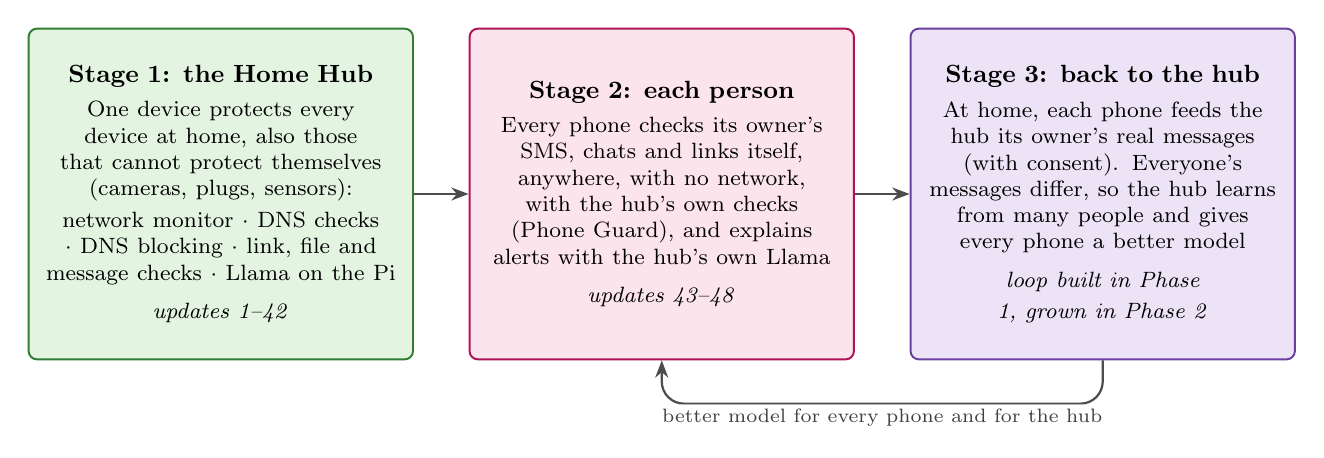
\begin{tikzpicture}[x=1cm,y=1cm]
  \node[pib, text width=4.6cm, minimum height=4.2cm, anchor=north] (s1) at (0,0)
    {\textbf{Stage 1: the Home Hub}\\[3pt]\footnotesize One device protects every device at home,
     also those that cannot protect themselves (cameras, plugs, sensors):\\[2pt]
     network monitor $\cdot$ DNS checks $\cdot$ DNS blocking $\cdot$ link, file and message checks $\cdot$
     Llama on the Pi\\[3pt] \textit{updates 1--42}};
  \node[phb, text width=4.6cm, minimum height=4.2cm, anchor=north] (s2) at (5.6,0)
    {\textbf{Stage 2: each person}\\[3pt]\footnotesize Every phone checks its owner's SMS, chats and links
     itself, anywhere, with no network, with the hub's own checks (Phone Guard), and explains alerts with
     the hub's own Llama\\[3pt] \textit{updates 43--48}};
  \node[adv, text width=4.6cm, minimum height=4.2cm, anchor=north] (s3) at (11.2,0)
    {\textbf{Stage 3: back to the hub}\\[3pt]\footnotesize At home, each phone feeds the hub its owner's
     real messages (with consent). Everyone's messages differ, so the hub learns from many people and
     gives every phone a better model\\[3pt] \textit{loop built in Phase 1, grown in Phase 2}};
  \draw[arr] (s1.east) -- (s2.west);
  \draw[arr] (s2.east) -- (s3.west);
  \draw[arr, rounded corners=8pt] (s3.south) -- ++(0,-0.55) -| node[lab, pos=0.25, below] {better model for every phone and for the hub} (s2.south);
\end{tikzpicture}
\caption{The three stages of Sajag. Stage 1 covers the whole home; stage 2 covers each person anywhere;
stage 3 lets each person's messages improve the protection of everyone.}
\label{fig:stages}
\end{figure}

\subsection{Stage 1: the Home Hub protects every device}

A home has more devices than people, and many of them, like a camera or a smart plug, can run no security
software. The only place that sees all of them is the network. So the first part we built was a hub: a
Raspberry Pi 4 that is the home's Wi-Fi hotspot and its DNS server. Every device's traffic passes through it,
so it can see a device scanning the network, calling a controller at fixed times, looking up random-looking
names or opening a phishing site, without installing anything on the device. Because it is the DNS server,
it can also \emph{protect}, not only detect: it refuses to resolve the websites of dangerous messages and of
phishing sites, for every device at once. The hub also checks messages, links and files sent to it from a
phone or from its web page, and runs Llama to explain every alert.

\subsection{Stage 2: protection for each person, on their own phone}

The hub protects only what is at home. Scam messages reach a person wherever they are, and a message has to be
judged when it arrives, not when the phone gets home. So the second part puts the hub's message and link
checks on each phone (Phone Guard): the same rules, the same model, the same thresholds, ported from the hub's
Python code to Kotlin and checked to give the same verdict on 16,272 messages. The phone then judges every SMS
in a few milliseconds, offline, and shows the alert at once. Finally the phone copies the hub's own Llama
file once and explains alerts itself when the hub cannot be reached: 3.6\,s on a Galaxy S25.

\subsection{Stage 3: each person's messages make everyone's protection better}

Every person receives a different set of messages: their banks, their mobile operator, their college or office,
their family's chats, the scams aimed at people like them. No public dataset has this range, and the public
data our first model learned from is mostly British and Western. Our tests show the cost: with text alone, the
model flags many normal Indian messages (Section~\ref{sec:results}).

So when a phone is home, it sends each message to the hub with its real sender ID. The hub adds what the phone
does not have (the 392,000-site phishing list, the file checks), answers at once, and, for phones whose owner
switched the study on, keeps the message in a log with every digit masked. The household then labels these
messages in the hub's terminal (fraud, marketing or normal). From them the hub trains the next model, compares
it with the current one under a rule fixed before the test, and, if it passes, exports it to every phone with
the same parity check that keeps phone and hub identical (Figure~\ref{fig:loop}).

\begin{figure}[H]
\centering
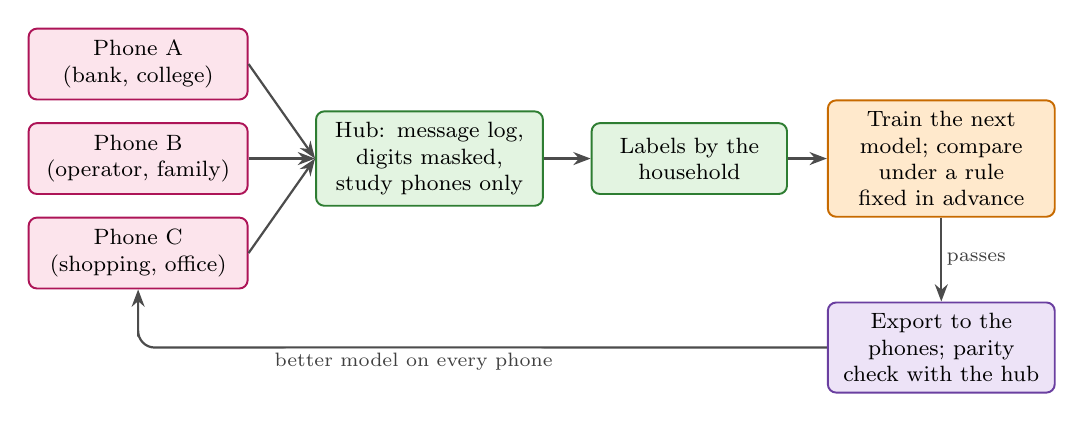
\begin{tikzpicture}[x=1cm,y=1cm, node distance=0.5cm]
  \node[phb, small, text width=2.5cm] (p1) at (0,1.2) {Phone A\\ (bank, college)};
  \node[phb, small, text width=2.5cm] (p2) at (0,0) {Phone B\\ (operator, family)};
  \node[phb, small, text width=2.5cm] (p3) at (0,-1.2) {Phone C\\ (shopping, office)};
  \node[pib, small, text width=2.6cm] (log) at (3.7,0) {Hub: message log, digits masked, study phones only};
  \node[pib, small, text width=2.2cm] (lab) at (7.0,0) {Labels by the household};
  \node[det, small, text width=2.6cm] (train) at (10.2,0) {Train the next model; compare under a rule fixed in advance};
  \node[adv, small, text width=2.6cm] (exp) at (10.2,-2.4) {Export to the phones; parity check with the hub};
  \foreach \p in {p1,p2,p3} \draw[arr] (\p.east) -- (log.west);
  \draw[arr] (log) -- (lab);
  \draw[arr] (lab) -- (train);
  \draw[arr] (train) -- node[lab, right] {passes} (exp);
  \draw[arr, rounded corners=6pt] (exp.west) -| node[lab, pos=0.3, below] {better model on every phone} (0,-2.05) -- (p3.south);
\end{tikzpicture}
\caption{Stage 3, the learning loop. Each phone's real messages, from a different corner of Indian life,
reach the hub; the model trained on them goes back to every phone.}
\label{fig:loop}
\end{figure}

\textbf{What Phase 1 built, and what it showed.} Every block of this loop exists and was run: the forwarding,
the log, the labelling and review tools, the training and comparison of SMS model v2 (three classes: fraud,
marketing, normal), and the export and parity check. On the team's three phones the hub received 2,674
messages; 121 were labelled in the first run. Model v2 cut the marketing and normal messages flagged from
registered sender IDs from 10 to 0 on held-out phones, but missed the one scam from a registered ID that v1
caught, so it did not pass the rule we had fixed in advance, and the phones keep v1
(Section~\ref{sec:smsv2}). The loop works; it needs more labelled messages, which is the first goal of
Phase 2, together with personal models and federated training so that texts need not leave the phone
(Section~\ref{sec:phase2}).

\subsection{Design principles}

\begin{enumerate}[label=\textbf{P\arabic*.}]
  \item \textbf{Small checkers decide, Llama explains.} Rules and small models give the verdict in
        milliseconds. A 1B model is slow on a Pi 4, can be wrong, and could be talked into ``safe'' by a
        scammer's text, so it never decides. It only explains, and its sentences are checked against the
        evidence it was given.
  \item \textbf{Nothing leaves the home network.} The phone decides on its own and talks to the hub over the
        hub's own Wi-Fi; neither needs an outside service for any check.
  \item \textbf{Two parts that also work apart.} The phone protects its owner anywhere; the hub protects every
        device at home. The phone runs the hub's own checks, so they agree.
  \item \textbf{Indian scams first:} TRAI sender IDs, \code{.bank.in}, \code{.gov.in}, Indian brands, KYC, UPI,
        OTP and APK scams, the 1930 helpline.
  \item \textbf{Answer at once, explain after.} The verdict and the playbook's steps appear immediately;
        Llama's explanation replaces them in the same alert seconds later.
  \item \textbf{Protect, not only detect:} scam websites are blocked on the hub's DNS, with an undo.
  \item \textbf{Measure on real hardware and real data,} and report the bad numbers too.
  \item \textbf{Defensive only.} No attack tools; the lab device's test modes are harmless imitations, and public
        malware traffic is replayed from files, never sent.
\end{enumerate}

% ================================================================= 4
\section{System architecture}
\label{sec:arch}

Figure~\ref{fig:arch} shows the whole system. Evidence comes in at the top: the phone's messages, the hub's
web page, and the traffic of the devices on the hub's Wi-Fi. Checkers judge it. Every checker writes the same
\textbf{finding}: a verdict (safe, suspicious or dangerous), a score from 0 to 1, a scam type and short reasons.
A score of 0.5 or more is suspicious and 0.8 or more is dangerous, for every checker, so the advisor never
needs to know which checker made a finding.

\begin{figure}[tb]
\centering
\resizebox{\textwidth}{!}{%
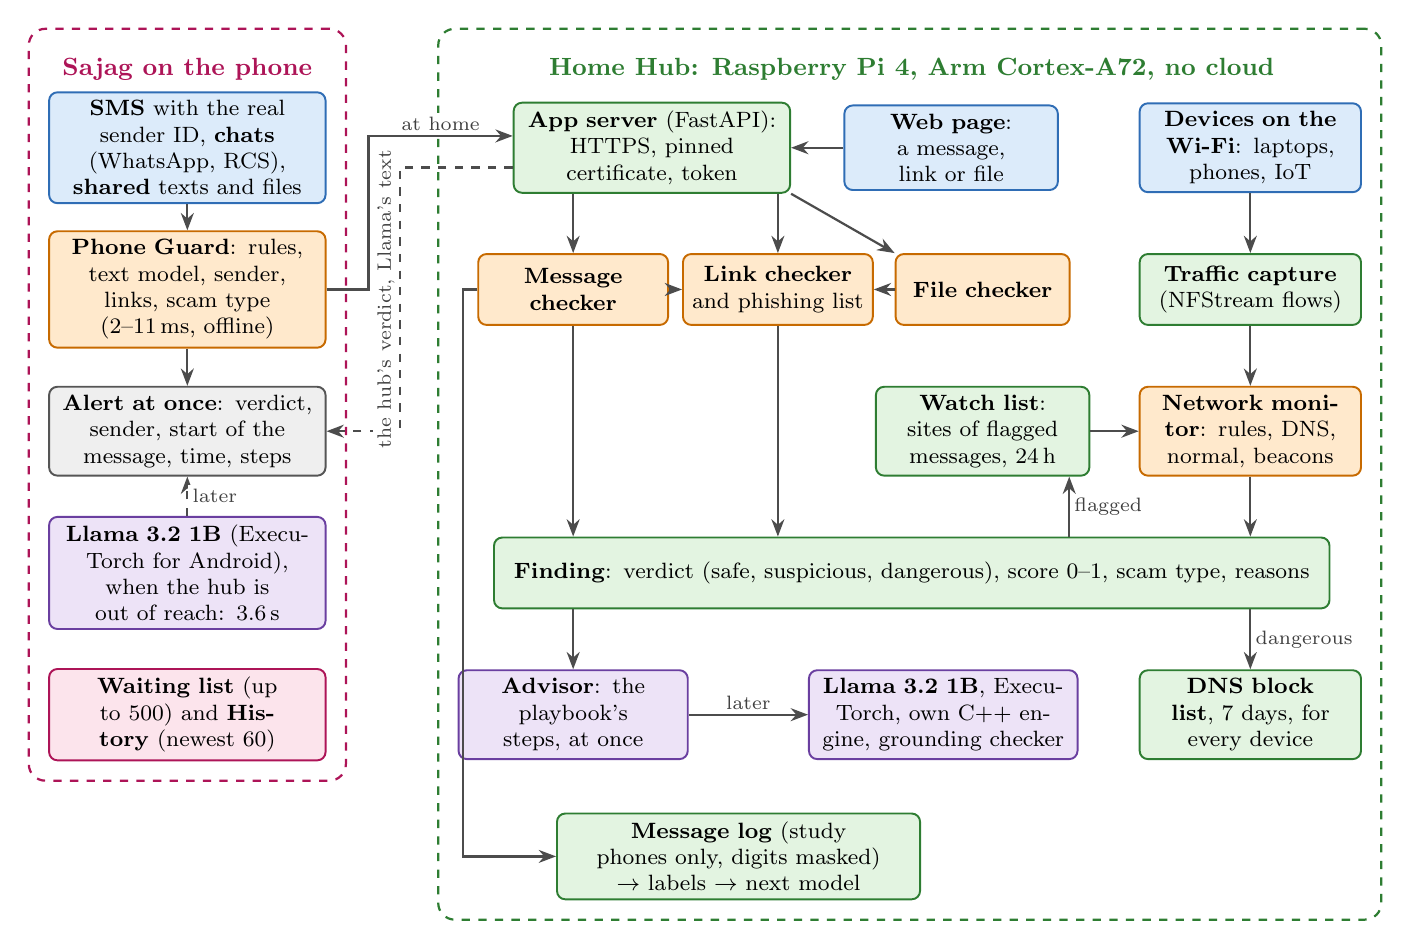
\begin{tikzpicture}[x=1cm,y=1cm, box/.append style={font=\footnotesize, inner sep=3pt}]
  % ---- titles
  \node[font=\small\bfseries, text=phLine] (tph) at (-6.6,1.0) {Sajag on the phone};
  \node[font=\small\bfseries, text=piLine] (thub) at (2.6,1.0) {Home Hub: Raspberry Pi 4, Arm Cortex-A72, no cloud};
  % ---- the phone
  \node[inp, text width=3.3cm] (in) at (-6.6,0) {\textbf{SMS} with the real sender ID, \textbf{chats} (WhatsApp, RCS), \textbf{shared} texts and files};
  \node[det, text width=3.3cm] (pg) at (-6.6,-1.8) {\textbf{Phone Guard}: rules, text model, sender, links, scam type (2--11\,ms, offline)};
  \node[outb, text width=3.3cm] (alert) at (-6.6,-3.6) {\textbf{Alert at once}: verdict, sender, start of the message, time, steps};
  \node[adv, text width=3.3cm] (pl) at (-6.6,-5.4) {\textbf{Llama 3.2 1B} (ExecuTorch for Android), when the hub is out of reach: 3.6\,s};
  \node[phb, text width=3.3cm] (wait) at (-6.6,-7.2) {\textbf{Waiting list} (up to 500) and \textbf{History} (newest 60)};
  % ---- the hub
  \node[pib, text width=3.3cm] (srv) at (-0.7,0) {\textbf{App server} (FastAPI): HTTPS, pinned certificate, token};
  \node[inp, text width=2.5cm] (page) at (3.1,0) {\textbf{Web page}: a message, link or file};
  \node[inp, text width=2.6cm] (devs) at (6.9,0) {\textbf{Devices on the Wi-Fi}: laptops, phones, IoT};
  \node[det, text width=2.2cm] (msg) at (-1.7,-1.8) {\textbf{Message checker}};
  \node[det, text width=2.2cm] (lnk) at (0.9,-1.8) {\textbf{Link checker} and phishing list};
  \node[det, text width=2.0cm] (fil) at (3.5,-1.8) {\textbf{File checker}};
  \node[pib, text width=2.6cm] (cap) at (6.9,-1.8) {\textbf{Traffic capture} (NFStream flows)};
  \node[pib, text width=2.5cm] (watch) at (3.5,-3.6) {\textbf{Watch list}: sites of flagged messages, 24\,h};
  \node[det, text width=2.6cm] (net) at (6.9,-3.6) {\textbf{Network monitor}: rules, DNS, normal, beacons};
  \node[pib, text width=10.4cm] (find) at (2.6,-5.4) {\textbf{Finding}: verdict (safe, suspicious, dangerous), score 0--1, scam type, reasons};
  \node[adv, text width=2.7cm] (quick) at (-1.7,-7.2) {\textbf{Advisor}: the playbook's steps, at once};
  \node[adv, text width=3.2cm] (llama) at (3.0,-7.2) {\textbf{Llama 3.2 1B}, ExecuTorch, own C++ engine, grounding checker};
  \node[pib, text width=2.6cm] (block) at (6.9,-7.2) {\textbf{DNS block list}, 7 days, for every device};
  \node[pib, text width=4.4cm] (log) at (0.4,-9.0) {\textbf{Message log} (study phones only, digits masked) $\to$ labels $\to$ next model};
  \begin{scope}[on background layer]
    \node[group=phLine, fit=(tph)(in)(pg)(alert)(pl)(wait)] {};
    \node[group=piLine, fit=(thub)(srv)(page)(devs)(msg)(lnk)(fil)(cap)(watch)(net)(find)(quick)(llama)(block)(log)] {};
  \end{scope}
  % ---- on the phone
  \draw[arr] (in) -- (pg);
  \draw[arr] (pg) -- (alert);
  \draw[later] (pl) -- node[lab, right] {later} (alert);
  \draw[arr] (pg.east) -- (-4.3,-1.8) -- (-4.3,0.15) -- node[lab, above] {at home} (srv.west |- 0,0.15);
  \draw[later] (srv.west |- 0,-0.25) -- (-3.9,-0.25) -- node[lab, rotate=90, above] {the hub's verdict, Llama's text} (-3.9,-3.6) -- (alert.east);
  \draw[arr] (page) -- (srv);
  \draw[arr] (msg.north |- srv.south) -- (msg.north);
  \draw[arr] (lnk.north |- srv.south) -- (lnk.north);
  \draw[arr] (srv.south east) -- (fil.north west);
  \draw[arr] (msg) -- (lnk);
  \draw[arr] (fil) -- (lnk);
  \draw[arr] (devs) -- (cap);
  \draw[arr] (cap) -- (net);
  \draw[arr] (watch) -- (net);
  \draw[arr] (msg.south) -- (msg.south |- find.north);
  \draw[arr] (lnk.south) -- (lnk.south |- find.north);
  \draw[arr] (net.south) -- (net.south |- find.north);
  \draw[arr] (4.6,0 |- find.north) -- node[lab, right] {flagged} (4.6,0 |- watch.south);
  \draw[arr] (quick.north |- find.south) -- (quick.north);
  \draw[arr] (quick) -- node[lab, above] {later} (llama);
  \draw[arr] (block.north |- find.south) -- node[lab, right] {dangerous} (block.north);
  \draw[arr] (msg.west) -- (-3.1,-1.8) |- (log.west);
\end{tikzpicture}}
\caption{The architecture of Sajag. Left: the phone, which judges every message itself and explains alerts
with Llama when the hub is out of reach. Right: the Home Hub, which checks what the phone sends and what its
page receives, watches every device on its Wi-Fi, blocks scam websites, explains alerts with Llama and keeps
the consented message log that trains the next model. Arrows never leave the home.}
\label{fig:arch}
\end{figure}

\subsection{One message, from arrival to explanation}

\begin{figure}[H]
\centering
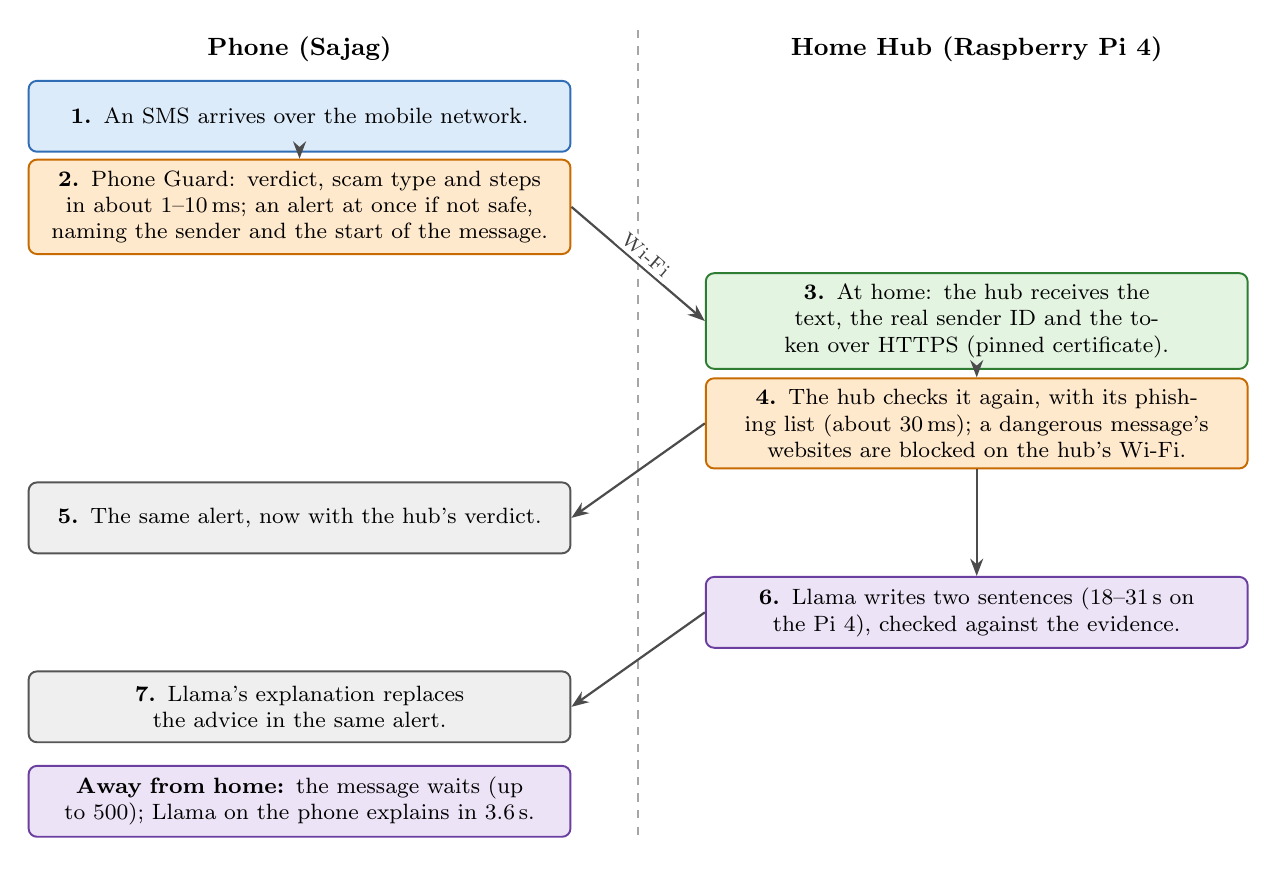
\begin{tikzpicture}[x=1cm,y=1cm]
  \node[font=\bfseries\small] at (-4.3,0.35) {Phone (Sajag)};
  \node[font=\bfseries\small] at (4.3,0.35) {Home Hub (Raspberry Pi 4)};
  \draw[dashed, black!35, line width=0.6pt] (0,0.6) -- (0,-9.7);
  \node[inp, small, text width=6.6cm] (a1) at (-4.3,-0.5) {\textbf{1.} An SMS arrives over the mobile network.};
  \node[det, small, text width=6.6cm] (a2) at (-4.3,-1.65) {\textbf{2.} Phone Guard: verdict, scam type and steps in about 1--10\,ms; an alert at once if not safe, naming the sender and the start of the message.};
  \node[pib, small, text width=6.6cm] (b1) at (4.3,-3.1) {\textbf{3.} At home: the hub receives the text, the real sender ID and the token over HTTPS (pinned certificate).};
  \node[det, small, text width=6.6cm] (b2) at (4.3,-4.4) {\textbf{4.} The hub checks it again, with its phishing list (about 30\,ms); a dangerous message's websites are blocked on the hub's Wi-Fi.};
  \node[outb, small, text width=6.6cm] (a3) at (-4.3,-5.6) {\textbf{5.} The same alert, now with the hub's verdict.};
  \node[adv, small, text width=6.6cm] (b3) at (4.3,-6.8) {\textbf{6.} Llama writes two sentences (18--31\,s on the Pi 4), checked against the evidence.};
  \node[outb, small, text width=6.6cm] (a4) at (-4.3,-8.0) {\textbf{7.} Llama's explanation replaces the advice in the same alert.};
  \node[adv, small, text width=6.6cm] (a5) at (-4.3,-9.2) {\textbf{Away from home:} the message waits (up to 500); Llama on the phone explains in 3.6\,s.};
  \draw[arr] (a1) -- (a2);
  \draw[arr] (a2.east) -- node[lab, above, sloped] {Wi-Fi} (b1.west);
  \draw[arr] (b1) -- (b2);
  \draw[arr] (b2.west) -- (a3.east);
  \draw[arr] (b2) -- (b3);
  \draw[arr] (b3.west) -- (a4.east);
\end{tikzpicture}
\caption{The path of one message. A chat follows the same path; a shared file goes to the hub's file checker.}
\label{fig:seq}
\end{figure}

\subsection{Where it runs}

\begin{figure}[H]
\centering
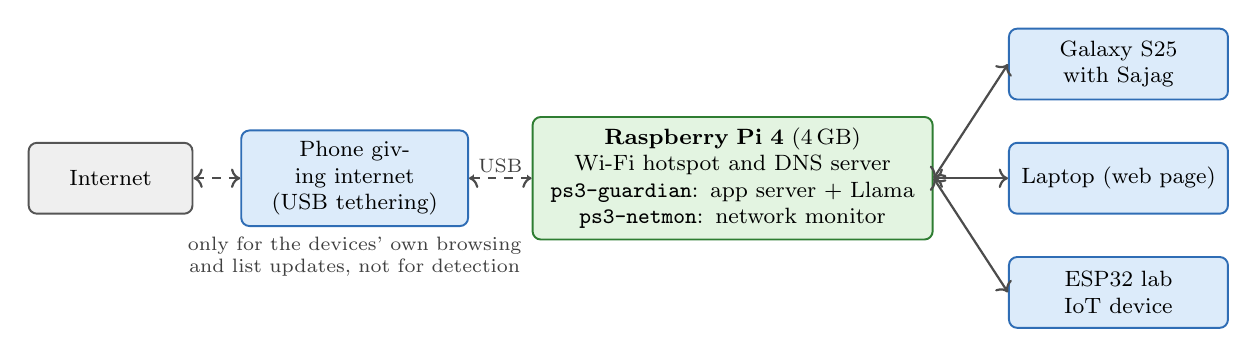
\begin{tikzpicture}[x=1cm,y=1cm]
  \node[outb, small, text width=1.8cm] (inet) at (-6.6,0) {Internet};
  \node[inp, small, text width=2.6cm] (up) at (-3.5,0) {Phone giving internet (USB tethering)};
  \node[pib, small, text width=4.8cm] (pi) at (1.3,0)
    {\textbf{Raspberry Pi 4} (4\,GB)\\ Wi-Fi hotspot and DNS server\\ \code{ps3-guardian}: app server + Llama\\ \code{ps3-netmon}: network monitor};
  \node[inp, small, text width=2.5cm] (s25) at (6.2,1.45) {Galaxy S25 with Sajag};
  \node[inp, small, text width=2.5cm] (lap) at (6.2,0) {Laptop (web page)};
  \node[inp, small, text width=2.5cm] (esp) at (6.2,-1.45) {ESP32 lab IoT device};
  \draw[arr, <->, dashed] (inet) -- (up);
  \draw[arr, <->, dashed] (up) -- node[lab, above] {USB} (pi);
  \foreach \d in {s25,lap,esp} \draw[arr, <->] (pi.east) -- (\d.west);
  \node[lab, below=2pt of up, text width=4.3cm, align=center] {only for the devices' own browsing and list updates, not for detection};
\end{tikzpicture}
\caption{The lab set-up. Solid lines (the hub's Wi-Fi) are all that detection needs; dashed lines (the
internet) are only for the devices' browsing and for refreshing the phishing list.}
\label{fig:where}
\end{figure}

\begin{table}[H]
\centering\small
\begin{tabularx}{\textwidth}{@{}>{\raggedright\arraybackslash}p{4.2cm}X@{}}
\toprule
\textbf{Device} & \textbf{Role}\\
\midrule
Raspberry Pi 4 Model B, 4\,GB & The Home Hub. Raspberry Pi OS Lite 64-bit (Debian 13), Python 3.13, booted from a USB 3.2 drive. Two systemd services: \code{ps3-guardian} (app server and Llama) and \code{ps3-netmon} (network monitor). Wi-Fi hotspot \code{PS3-Guardian-Lab} (10.42.0.1) and its DNS server\\
Samsung Galaxy S25 and teammates' Android phones & Sajag: Phone Guard, Llama on the phone, alerts, network alerts, sharing files and texts to the hub\\
ESP32 DevKit on an IoT Pro Kit & A small IoT device on the lab Wi-Fi (DHT11, BMP180 readings every 15\,s), with harmless test modes that imitate an infected device\\
A second phone on the Pi's USB port & Gives the Pi internet by USB tethering, only for the devices' browsing\\
Laptop & Opens the hub's page; exports the model, builds the C++ engine (WSL2) and the Android app\\
\bottomrule
\end{tabularx}
\caption{Hardware.}
\end{table}

% ================================================================= 5
\section{Algorithms and components}
\label{sec:algo}

\subsection{Message checker (SMS and chats)}
\label{sec:sms}

The message checker turns a message and its sender into one score from 0 to 1, in steps that each raise or
lower it. It runs on the hub (\code{home-hub/detectors/sms/}, Python) and on the phone (\code{guard/}, Kotlin), with the
same rules, model weights and thresholds.

\textbf{1. Red-flag rules for India} (\code{rules\_india.py}). Regular expressions for the signs Indian scams use:
KYC, OTP, UPI, an \code{.apk} file, urgency (``blocked today'', ``within 24 hours''), money and prizes, a bank's or
the government's name with a link not on \code{.bank.in} or \code{.gov.in}, talk of an OTP, PIN or password, and
whether the message asks you to share one (with a negation check: ``do not share'' is not a request). They give
the reasons shown to the user and 11 numeric features for the model.

\textbf{2. Text model} (\code{train\_baseline.py}). The text is cleaned (HTML entities, mis-encodings, look-alike
characters) and cut into character n-grams of 2 to 5 letters within word boundaries (TF-IDF, at most 20,000
features), joined with the 11 rule features; a class-balanced logistic regression gives the probability $p$ that
the message is a threat. It was trained on 70\% of 6,053 unique public messages (UCI SMS Spam Collection and
Mishra \& Soni) and reached F1 0.950 on the other 30\%.

\textbf{3. Sender ID.} In India, TRAI's rules make businesses send from registered headers such as
\code{JD-HDFCBK-S}, whose suffix says the kind of message. The phone reads the real header of every SMS. The
score is changed in odds space, so that each piece of evidence multiplies the odds of fraud:
\begin{equation}
  o = \frac{p}{1-p}, \qquad o' = o \cdot m_{\text{sender}} \cdot m_{\text{links}}, \qquad s = \frac{o'}{1+o'}
\end{equation}
with $m_{\text{sender}} = 0.02$ for a service, transactional or government header (\code{-S}, \code{-T},
\code{-G}), $0.1$ for a promotional one (\code{-P}), and $4$ for a personal mobile number whose message has a link,
money, urgency, bank words or OTP talk. The multipliers follow TRAI's rules and were set before any test, not
fitted to one.

\textbf{4. Links.} Every link goes to the link checker (Section~\ref{sec:links}): $m_{\text{links}} = 3$ for a
dangerous link, $1.5$ for a suspicious one, $0.3$ if every link is on an official site. An \code{.apk} link, a site
on the phishing list or a brand's name on someone else's site makes the message dangerous whoever sent it.

\textbf{5. Sender rules} (update 37), measured on the hub before being switched on. A registered header can make a
scam look safe, so: \emph{cap}: no header can bring below 0.5 a message that asks you to share an OTP or PIN (and
scored $\ge 0.5$ before the sender), or that names a bank, payment app or government body with a link the link
checker does not call safe; \emph{brand}: a risky message that names a bank or payment app, sent from a header
that belongs to none of the named brands, gets no reduction from its header.

\textbf{6. Verdict, scam type and what the message says.} $s \ge 0.8$ is dangerous, $s \ge 0.5$ suspicious. Ordered
rules choose the scam type, and with it the playbook (\code{home-hub/advisor/categorize.py}: APK, digital arrest, delivery
fee, job task, lottery or reward, utility disconnection, OTP theft, bank KYC, phishing link, general). The
organisation the message claims to be is taken from a fixed list of 157 domains of 33 brands
(\code{brands.py}), never from the message. Since prompt v5 (update 47), 24 more patterns name, in fixed words,
what a flagged message itself says: its claim (``says your electricity will be cut off''), the amount
(``mentions \rupee{}25,000''), a deadline (``says you must act now'') and what it asks (``asks you to pay money'',
``has a link to open''), at most four (\code{says.py}).

\begin{algorithm}[H]
\caption{Verdict for one message (hub and phone)}
\KwIn{text $t$, sender $h$ (registered header, mobile number, name or none)}
\KwOut{verdict, score $s$, scam type, reasons, what the message says}
$t \leftarrow$ \textsc{Clean}($t$)\;
$R, \mathbf{f} \leftarrow$ \textsc{IndiaRules}($t$) \tcp*{reasons and 11 features}
$p \leftarrow$ \textsc{LogReg}(\textsc{CharNGrams}$_{2..5}$($t$) $\Vert$ $\mathbf{f}$)\;
$L \leftarrow$ [\textsc{CheckLink}($u$) for each link $u$ in $t$]\;
\lIf{any $\ell \in L$ is decisive (\code{.apk}, listed, brand on another site)}{\Return dangerous}
$o \leftarrow \frac{p}{1-p} \cdot m_{\text{sender}}(h, R) \cdot m_{\text{links}}(L)$\;
\If{\textsc{Cap}($t, R, L, p$)}{$o \leftarrow \max(o, 1)$ \tcp*{no header clears an OTP request or a bank link}}
$s \leftarrow o / (1+o)$\;
verdict $\leftarrow$ dangerous if $s \ge 0.8$, suspicious if $s \ge 0.5$, else safe\;
\If{verdict $\neq$ safe}{type $\leftarrow$ \textsc{ScamType}($t, R$);\; says $\leftarrow$ \textsc{WhatItSays}($t$)}
\Return verdict, $s$, type, $R$, says\;
\end{algorithm}

\textbf{Chats.} WhatsApp and RCS chats never reach other apps as messages, but their notifications do. With
notification access, Sajag reads the newest incoming message of a chat notification, only from senders shown as a
phone number (not your contacts). A message is known by its app, sender, text and the time its app gives it, so a
notification posted again is checked once but the same words sent again are checked again (app 3.2). One
exception for contacts: a message that names an app file (\code{Wedding\_Invitation.apk}) is checked even from a
contact, and only the file's name is sent.

\subsubsection*{SMS model v2: the learning loop, tested}
\label{sec:smsv2}

Model v2 (\code{train\_v2.py}) has three classes, fraud, marketing and normal, and learns from the public data plus
the team's labelled messages; marketing is trusted only from registered headers. Near-copies of the India test set
never train it. Before the comparison we fixed a rule: v2 replaces v1 only if, as the app decides, it catches at
least as many India-set scams (minus two), and on each phone held out in turn it flags fewer normal and marketing
messages and misses no more scams. In the second run (94 different labelled team messages) v2 cut the normal and
marketing messages flagged from registered headers on held-out phones from 10 to 0, but missed the one scam from a
registered header that v1 caught. It did not pass, and the phones keep v1. The loop is in place; it needs more
labelled messages.

\subsection{Link checker}
\label{sec:links}

About a millisecond per link, with no network (\code{home-hub/detectors/url/}).

\begin{enumerate}
  \item \textbf{Read the address} with an offline public-suffix list: the registered domain
        (\code{sbi.co.in.kyc-check.xyz} is really \code{kyc-check.xyz}), punycode, and sites hidden in Google
        redirects, Google Translate and AMP links.
  \item \textbf{Sure signs} (dangerous): an \code{.apk} file; the ``@'' trick; a site on the phishing list
        (Phishing.Database, about 392,000 live phishing domains in SQLite on the hub); a brand's name on someone
        else's site with sign-in words, a cheap ending, free hosting or a fake prefix.
  \item \textbf{Says nothing by itself}: short links, chat links, shared documents and forms. The sender and the
        text decide.
  \item \textbf{Official} (safe): \code{.bank.in}, \code{.gov.in}, \code{.nic.in}, \code{.fin.in}, brand endings
        (\code{.sbi}) and 157 domains of 33 brands and organisations.
  \item \textbf{Otherwise the domain model}: logistic regression on hashed 2--5-letter pieces of the registered
        domain ($2^{18}$ features) and 7 numbers (length, digits, hyphens, letter entropy, vowels, consonant runs,
        ending), trained on 996,256 domains (PhiUSIIL, Phishing.Database, Chrome UX Report top sites). Its odds
        are then multiplied for what it cannot see: an IP address $\times 6$, a brand's name $\times 5$ ($\times 3$
        in a subdomain), look-alike letters $\times 3$, sign-in words $\times 2$, many subdomains $\times 1.5$, one
        of the 10,000 most visited sites $\times 0.1$.
\end{enumerate}

\textbf{Why only the domain:} in the main public dataset every legitimate URL is a bare home page and phishing URLs
have paths; a model reading whole URLs learns ``a path means phishing'', and every genuine SMS link has a path.
Rules handle paths instead.

\subsection{File checker}
\label{sec:files}

About 20\,ms per file on the hub; the file stays in memory and is never stored, opened in a reader or run
(\code{home-hub/detectors/files/}).
\begin{itemize}
  \item \textbf{What is it really?} The first bytes say what a file is, whatever its name: an app named
        \code{Invitation.pdf}, a double ending (\code{Card.pdf.apk}) or a hidden right-to-left character is a disguise.
  \item \textbf{APK}: dangerous when it comes in a chat; permissions OTP thieves need are named (read SMS, control
        the screen, read notifications).
  \item \textbf{PDF}: JavaScript that runs on opening, launch commands, embedded files (checked too), read only from
        the PDF's dictionaries and object streams. Harmless scripts are recognised (Acrobat form helpers, page jumps,
        KiCad schematic menus by a fingerprint of KiCad's own script).
  \item \textbf{Office}: macros, remote templates and objects, DDE, programs in embedded objects.
  \item \textbf{Zip}: password locks, apps inside, up to 20 inner files checked; limits against zip bombs
        (25\,MB per file, 50\,MB unpacked).
  \item \textbf{Saved web pages}: a password box (a fake sign-in page that needs no website), redirects, scripts.
  \item \textbf{Links} in any file go to the link checker.
\end{itemize}

\subsection{Network monitor}
\label{sec:net}

The hub is the Wi-Fi hotspot, so every device's traffic passes through it. NFStream turns packets into
\textbf{flows} (addresses, ports, bytes, packets, duration, server name). The monitor reads who talks to whom, when
and how much, never the content (\code{home-hub/detectors/net/}, service \code{ps3-netmon}).

\begin{table}[H]
\centering\small
\begin{tabularx}{\textwidth}{@{}>{\raggedright\arraybackslash}p{3.3cm}X@{}}
\toprule
\textbf{Detector} & \textbf{Rule (per device, sliding windows)}\\
\midrule
Port scan & $\ge 20$ ports tried without an answer within 60\,s (100 ports: dangerous)\\
Network sweep & $\ge 15$ machines tried on one port within 60\,s, more unanswered than answered; Telnet: dangerous (Mirai)\\
Flood, slow DoS & $\ge 300$ flows or $\ge 200$ SYN-only flows to one service within 10\,s; $\ge 50$ long near-empty flows within 60\,s\\
Password guessing & $\ge 15$ short flows to a login port (SSH, FTP, Telnet, mail, databases) within 60\,s\\
Risky ports & a home device connecting out on Telnet, IRC, Tor, SMB or 4444\\
Beacon & $\ge 10$ new connections to one server $\ge 30$\,s apart with a coefficient of variation of the gaps below 0.15, only to servers outside the device's normal\\
Phishing look-up & a looked-up name that the link checker finds decisive or listed\\
DGA names & $\ge 5$ names scored $\ge 0.9$ by a DGA model (character n-grams, trained on 800,000 names) within 10\,min\\
DNS tunnel & $\ge 25$ unique sub-names of $\ge 18$ characters under one domain within 10\,min\\
Device's normal & per 5 minutes: connections, bytes, servers, ports, look-ups; after 2\,h of learning, a value above $\max(3 \times p_{99}, \text{floor})$ with $\ge 5$ new servers; only devices with at most 50 usual servers (IoT, not laptops)\\
Scam link opened & a device looks up a site from a message flagged in the last 24\,h (the watch list)\\
\bottomrule
\end{tabularx}
\caption{The network detectors. The same problem is reported once per 10 minutes per device and peer, unless its score rises.}
\end{table}

For a beacon, with $\Delta_1,\dots,\Delta_{n-1}$ the gaps between $n$ new connections from a device to one server,
\begin{equation}
  \text{beacon} \iff n \ge 10,\quad \min_i \Delta_i \ge 30\,\text{s},\quad \frac{\sigma(\Delta)}{\mu(\Delta)} < 0.15,
  \quad \text{server} \notin \text{normal(device)}.
\end{equation}
Only new connections count: keep-alives inside one open connection, split by NFStream's 10\,s idle timeout, once
looked like beacons (a false alarm we found and fixed on the lab Wi-Fi).

\textbf{Messages meet network traffic.} When a message is flagged, the hub puts the websites of its links on a
\textbf{watch list} for 24 hours. If any device then looks one up, the monitor raises ``Link from a scam message
opened''. This catches what the link checker alone rates safe: real Indian scams use short domains that look like
genuine bulk-SMS link domains, and the sender and the text gave them away.

\textbf{DNS blocking} (protection, not only detection). The hub is its hotspot's DNS server, so it refuses to resolve
the websites of dangerous messages, phishing sites a device looked up, and scam links a device opened, for 7 days,
for every device; websites blocked by hand stay blocked until unblocked. Official, popular and shared sites are never
blocked. The app only writes a list; a small root helper, run by systemd whenever the list changes, keeps only valid
names and makes dnsmasq answer NXDOMAIN for each. The set-up script undoes itself after 10 minutes unless confirmed,
so a wrong setting cannot lock anyone out.

\textbf{Each device's risk.} Every device gets AT RISK, CHECK or OK from its alerts of the last 24 hours, on the page
and in the app.

\subsection{Advisor and Llama}
\label{sec:llama}

\begin{figure}[H]
\centering
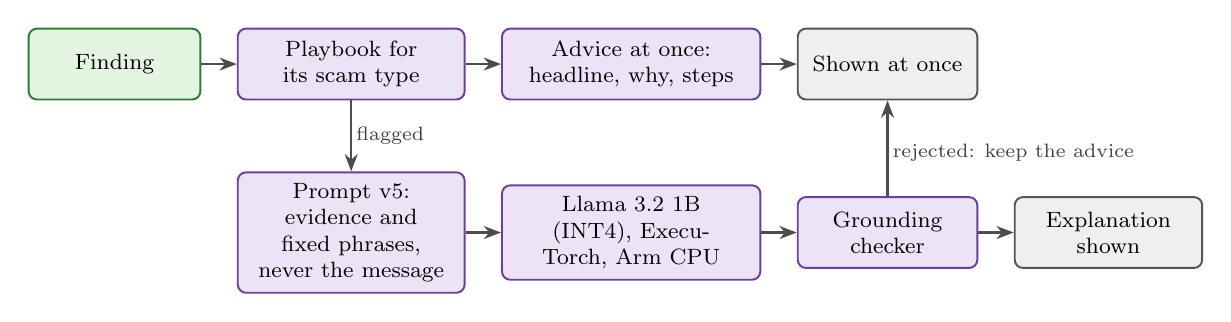
\begin{tikzpicture}[node distance=0.45cm]
  \node[pib, small, text width=1.9cm] (f) {Finding};
  \node[adv, small, text width=2.6cm, right=of f] (p) {Playbook for its scam type};
  \node[adv, small, text width=3.0cm, right=of p] (q) {Advice at once: headline, why, steps};
  \node[outb, small, text width=2.0cm, right=of q] (s1) {Shown at once};
  \node[adv, small, text width=2.6cm, below=0.9cm of p] (pr) {Prompt v5: evidence and fixed phrases, never the message};
  \node[adv, small, text width=3.0cm, right=of pr] (l) {Llama 3.2 1B (INT4), ExecuTorch, Arm CPU};
  \node[adv, small, text width=2.0cm, right=of l] (v) {Grounding checker};
  \node[outb, small, text width=2.1cm, right=of v] (s2) {Explanation shown};
  \draw[arr] (f) -- (p); \draw[arr] (p) -- (q); \draw[arr] (q) -- (s1);
  \draw[arr] (p) -- node[lab, right] {flagged} (pr);
  \draw[arr] (pr) -- (l); \draw[arr] (l) -- (v); \draw[arr] (v) -- (s2);
  \draw[arr] (v.north) -- node[lab, right, pos=0.45] {rejected: keep the advice} (v.north |- q.south);
\end{tikzpicture}
\caption{The advisor: the top row is instant; the bottom row runs in the background.}
\label{fig:adv}
\end{figure}

\textbf{Playbooks} (\code{home-hub/advisor/playbooks/*.md}): 25 short files, 11 for messages and links, 3 for files, 11 for the
network. Each has a title, a severity, the steps to take (for scams: the 1930 helpline and cybercrime.gov.in), and
three lines only Llama sees: who the scam pretends to be, what it wants, and one checked fact. \emph{The steps users see
always come from the playbook, word for word.}

\textbf{The prompt} (\code{prompt.py}, version 5) holds a fixed system text with worked examples (English and Hindi), then
the case: the scam type, what the scammer wants, the checked fact, the scanner's result, who the message pretends to be
(from the fixed list), what the message says (fixed phrases) and the warning signs. It never holds the message text or
the sender, so a scammer's words cannot steer Llama. A 1B model copies examples far better than it follows instructions,
so the examples carry the style. Network alerts have their own prompt and examples.

\begin{keybox}[title=Example: the case Llama is shown (prompt v5) and its answer]
\small\ttfamily
Scam type: Electricity disconnection scam\\
Scammer wants: to make you pay a fake bill or install a remote-control app\\
Fact: Real electricity companies send notices with the bill and do not ask you to call a personal number.\\
Scanner result: scam (high confidence)\\
Pretends to be: your electricity company\\
The message:\\
- says your electricity will be cut off\\
- says you must act now\\
- asks you to call or message someone\\[4pt]
\normalfont\itshape
This message pretends to be from your electricity company and says your power will be cut off soon unless you call a
number, to scare you into paying a scammer. Real electricity companies send notices with the bill and do not ask you to
call a personal number.
\end{keybox}

\textbf{The model.} Llama 3.2 1B Instruct, Meta's SpinQuant INT4 checkpoint, exported with ExecuTorch 1.5
(\code{export\_llm}, XNNPACK): 4-bit weights in groups of 32 with 8-bit dynamic activations, 8-bit embeddings and output
layer, a KV cache, the custom SDPA operator, 2,048 tokens of context; the \code{.pte} file is about 1.0\,GB. The same
file runs on the hub and on the phone.

\subsubsection*{Our C++ engine for the Pi 4}
\label{sec:engine}

ExecuTorch's prebuilt Python wheel stopped on the Pi 4 with ``Illegal instruction''. Disassembling its libraries with our
own tool (\path{home-hub/llama-engine/tools/check_arm_isa.py}) showed 43 Armv8.1 atomic instructions in the custom LLM operators,
built for Armv8.2; the Cortex-A72 is Armv8.0. We built our own engine (\code{home-hub/llama-engine/advisor\_server/}) with the Arm GNU
toolchain 14.3 and \code{-march=armv8-a -mtune=cortex-a72}, per file. It:
\begin{itemize}
  \item keeps the model loaded (loading takes 13.7\,s);
  \item reads the fixed start of the prompt (system text and examples, about 512 tokens, 38.5\,s) once, and reuses
        it from the KV cache for every alert;
  \item reads the rest in fixed 32-token pieces at fixed positions: kernels round differently by call length, and
        without this, the same alert could get a slightly different answer after a different earlier alert
        (checked by CRC-32 of the logits);
  \item decodes greedily, at most 80 new tokens in English and 192 in Hindi, and stops after two sentences;
  \item saves answers, so a repeated alert is explained at once.
\end{itemize}
A new explanation takes 18--31\,s on the Pi 4 (decode 3.3 tokens/s). ExecuTorch's own runner,
\code{llama\_main}, took 42.5\,s, because it also loaded the model for each alert.

\textbf{The grounding checker} (\code{validator.py}) runs before anyone sees an answer. It rejects an answer that
contradicts the verdict (``this is safe'') or is in the wrong language; drops any sentence with a phone number or link not
on an allowlist; keeps at most two complete sentences; and holds every sentence to its evidence: a sentence is dropped if
it has a number or names an organisation the case does not have, says ``never'' or ``always'' where the case does not,
claims where the message's link goes, or states a rule about what real companies do that the case's fact does not state.
If the answer is rejected, the playbook's advice stays.

\begin{algorithm}[H]
\caption{Explanation of one alert}
\KwIn{finding $F$ (not safe), language $\lambda$}
$B \leftarrow$ \textsc{Playbook}($F$.type);\; \textsc{Show}(\textsc{Advice}($B$, $F$)) \tcp*{at once}
$C \leftarrow$ \textsc{Case}($B$.facts, $F$.result, $F$.claims, $F$.says, $F$.reasons) \tcp*{never the message}
\lIf{$C$ in saved answers}{$A \leftarrow$ saved($C$)}
\Else{
  \tcp{prefix (system + examples) already in the KV cache}
  feed $C$ in 32-token pieces at fixed positions;\;
  $A \leftarrow$ greedy decode until two sentences or $N_{\max}(\lambda)$ tokens\;
}
$A' \leftarrow$ \textsc{Ground}($A$, $C$, $F$.verdict, $\lambda$) \tcp*{drop unsupported sentences}
\lIf{$A'$ is accepted}{\textsc{Show}($A'$) in the same alert}
\end{algorithm}

\subsection{Sajag on the phone: Phone Guard and Llama}
\label{sec:phone}

\textbf{Phone Guard} (update 43) runs the hub's message and link checks on the phone. Rather than writing new rules,
\code{home-hub/scripts/export\_phone\_guard.py} exports the hub's own data (the text model's vocabulary and weights, the India
rules' patterns, the brands, the sender odds and rules, the link model, the top sites, the scam types, the playbooks and
the prompt's examples) to \code{assets/guard/}, and a Kotlin port runs it: Python's regular expressions translated to
Java's, Python's text cleaning (HTML unescape, encoding fixes) and the public-suffix rules re-implemented, MurmurHash3 as
scikit-learn uses it, and the logistic regressions summed in the same order. A computer harness runs the phone's Kotlin
code on 16,272 messages and compares it with the hub's Python code field by field
(\code{home-hub/scripts/check\_phone\_guard.py}): same verdict on all 16,272, identical in every detail on 16,264 (the 8 others are
mis-encoded texts), and the same Llama prompt on all 8,833 that Llama explains. A message takes 2--11\,ms on the S25.

\textbf{Llama on the phone} (update 44). Llama's weights are not in the app (Meta's licence): a paired phone copies the
hub's own \code{.pte} and tokenizer once (\code{GET /llama}, over the pinned HTTPS connection, resumable, SHA-256
checked), and runs them with ExecuTorch 1.5.1's Android library on the phone's Arm CPU (XNNPACK) when the hub cannot be
reached, with the same prompt and the same grounding checker. On the Galaxy S25 an explanation takes 3.6\,s (5.2\,s when
the model loads first): the 678-token prompt is read at about 340 tokens/s, and 54 tokens are written at about 36
tokens/s. The model leaves memory after 3 idle minutes.

\textbf{The app} (Sajag 3.2): Home, Alerts, Network and Settings pages; a screen for every alert (what is happening, what
to do now with 1930 and cybercrime.gov.in, why it was flagged, the message with its links broken); notifications that name
the sender, the start of the message and the time it arrived, with nothing of it on a locked screen; a set-up in three
steps; and a waiting list of up to 500 messages for the hub.

\begin{algorithm}[H]
\caption{A message on the phone, at home or away}
\KwIn{message $m$ (SMS or chat) with sender $h$}
$F_p \leftarrow$ \textsc{PhoneGuard}($m$, $h$) \tcp*{1--10\,ms, offline}
\lIf{$F_p$ not safe}{\textsc{Notify}(sender, start of $m$, time, $F_p$, steps)}
\eIf{the hub answers (HTTPS, pinned, token)}{
  $F_h \leftarrow$ \textsc{Hub}($m$, $h$) \tcp*{adds the phishing list; may block sites}
  update the alert with $F_h$; later replace its text with the hub's Llama explanation\;
}{
  keep $m$ in the waiting list (up to 500)\;
  \lIf{$F_p$ not safe and Llama is on the phone}{\textsc{Notify}(\textsc{Explain}($F_p$)) \tcp*{3.6\,s}}
}
\end{algorithm}

\subsection{Security, privacy and safety}
\label{sec:privacy}

\begin{itemize}
  \item \textbf{No cloud.} Verdicts need no network; phone and hub talk only over the hub's Wi-Fi.
  \item \textbf{HTTPS with a pinned certificate} (the phone pins the hub's certificate fingerprint when pairing) and a
        128-bit pairing token on every request; repeated wrong tokens are refused for a minute.
  \item \textbf{What the hub keeps:} message texts only for phones whose owner switched the study on, with every digit
        masked; a safe message from a phone number is never stored; files are never stored (type, size and verdict only);
        network data is counts and server names, never contents.
  \item \textbf{Llama never sees the message}, only checked evidence and fixed phrases. Reasons never contain the
        sender's links or names. The grounding checker drops any number, link or organisation Llama makes up.
  \item \textbf{Users' steps come from playbooks} written from official Indian advice (1930, cybercrime.gov.in), never
        from the model.
  \item \textbf{Consent and undo.} Teammates who installed the app agreed to what the hub keeps and can switch the study
        off at any time; a website blocked by mistake is unblocked in one tap.
  \item \textbf{Defensive only.} No attack or traffic-generation tools; the ESP32's test modes and the test files only
        imitate harmful behaviour; public malware traffic (IoT-23) is replayed from files.
  \item \textbf{Licences.} Model weights are not in the repository or the app; lists whose terms forbid redistribution
        are not downloaded automatically.
\end{itemize}

% ================================================================= 6
\section{Implementation on Arm, and the problems we solved}
\label{sec:impl}

\begin{table}[H]
\centering\small
\begin{tabularx}{\textwidth}{@{}>{\raggedright\arraybackslash}p{3.1cm}X@{}}
\toprule
\textbf{Part} & \textbf{Software}\\
\midrule
Hub services & Python 3.13, FastAPI and uvicorn (HTTPS), scikit-learn, NumPy, tldextract, NFStream 6.6, SQLite, systemd, NetworkManager, dnsmasq\\
Llama & ExecuTorch 1.5 (\code{export\_llm}, XNNPACK), our C++ engine built with the Arm GNU toolchain 14.3 for the Cortex-A72; ExecuTorch Android 1.5.1 on the phone\\
Phone & Kotlin, Android 8.0+ (target API 36), WorkManager, NotificationListenerService; 38 Kotlin files, about 5,500 lines\\
IoT lab device & ESP32 DevKit (Arduino), DHT11 and BMP180\\
Tests & 379 automated tests (pytest), a Kotlin compile check with warnings as errors, a JVM harness for Phone Guard, an ESP32 simulation\\
\bottomrule
\end{tabularx}
\caption{Software. The repository has 66 Python files (about 12,700 lines), the Android app, the C++ engine and the ESP32 sketch.}
\end{table}

\textbf{How the work was delivered.} The hub is a real device on a real Wi-Fi, so every change reached it as a tested git
bundle, pulled on the Pi and pushed to GitHub: 53 numbered updates between 19 October and 22 November 2026. Every update
ran the full test suite first, and every result in this report comes from a script in the repository.

\textbf{Problems we solved along the way.}
\begin{enumerate}
  \item \textbf{ExecuTorch on an Armv8.0 CPU.} The prebuilt wheel crashed with ``Illegal instruction''; we found the
        Armv8.1 atomics with our own disassembly tool and built our own engine per file for \code{armv8-a}
        (Section~\ref{sec:engine}).
  \item \textbf{Llama too slow per alert} (42.5\,s with \code{llama\_main}, 11.7\,s of it loading): a resident model,
        a cached prompt prefix, two-sentence answers and saved answers brought a new alert to 18--31\,s and a repeat to
        zero.
  \item \textbf{Reused KV cache changed answers slightly}, because kernels round differently by call length: prompts
        are now read in 32-token pieces at fixed positions, and the same prompt gives the same logits (CRC-32 checked).
  \item \textbf{A 1B model invents things}, and the first checker only caught forbidden forms. We added grounding checks
        and graded 100 answers sentence by sentence; reading them also showed faults in the checks themselves (an ``OTP''
        example that failed its own check, \code{.bank.in} turned around), which we fixed.
  \item \textbf{Text-only scoring flagged most normal Indian messages} (64\% of the India set's normal messages): the
        phone now reads the real sender ID, which is what TRAI's headers are for.
  \item \textbf{A whole-URL phishing model learned ``a path means phishing''} from its dataset; the model now reads only
        the domain and rules handle paths.
  \item \textbf{False beacons on the lab Wi-Fi}: keep-alives in open connections, split by the flow timeout, looked like
        check-ins; only new connections count now. A busy hour on the lab Wi-Fi gave 5 false alarms (a port-443 sweep, an
        AMP cache and Gravatar on the phishing list, a laptop's ``unusual'' surge); after the fixes, 0 in 20,960 flows.
  \item \textbf{A capture that stopped silently} for two days made a false-alarm count meaningless: the monitor now
        counts watched time in 5-minute ticks, detects a stuck capture and restarts it.
  \item \textbf{Excel rewrote dates in the labelling sheet} and broke the per-day counts: labelling moved into the hub's
        terminal.
  \item \textbf{The S25 refused USB tethering to the Pi}: another phone gives the Pi internet, and the S25 joins the hub's
        Wi-Fi like any device.
  \item \textbf{The phone and the hub had to agree exactly}: a field-by-field parity harness on 16,272 messages found one
        porting bug (a missing odds factor for shared hosting), fixed before release.
  \item \textbf{The same chat message twice gave one alert}: a notification posted again and a new message with the same
        words looked alike; a message is now known by the time its app gives it.
\end{enumerate}

% ================================================================= 7
\section{Results}
\label{sec:results}

All numbers are measured with scripts in the repository, except where marked as a projection. Shares in brackets are
95\% Wilson intervals. ``Flagged'' means suspicious or dangerous: the app shows an alert.

\subsection{Accuracy test: scam and normal messages}
\label{sec:acc}

Run on 22 November with the phone's model and rules (the phone's Kotlin code gives the same verdicts as this Python code
on all 16,272 comparison messages, so these are the phone's numbers), without the hub's phishing list, as on the phone.

\begin{table}[H]
\centering\small
\begin{tabularx}{\textwidth}{@{}>{\raggedright\arraybackslash}X>{\raggedright\arraybackslash}p{3.6cm}>{\raggedright\arraybackslash}p{3.5cm}@{}}
\toprule
\textbf{Set} & \textbf{Scams flagged} & \textbf{Normal flagged}\\
\midrule
\textbf{Fishing for Smishing, India}: 859 scam campaigns reported by the public from Indian mobile numbers (one message per campaign); never used to build Sajag (the 80 messages of this dataset in our India set, and anything like them, left out) & \textbf{755 of 859 (87.9\%, 86--90\%)} & no normal messages\\
Public messages the model never trained on (1,816: UCI and Mishra \& Soni) & 304 of 318 (95.6\%, 93--97\%) & 18 of 1,498 (1.2\%, 1--2\%)\\
India test set (227 real messages; senders typed into the sheet; used while building the rules) & 96 of 100 (96.0\%, 90--98\%) & 44 of 75 (58.7\%, 47--69\%)\\
\quad with a real registered sender ID & -- & 1 of 10\\
\quad with a typed name (``Airtel'', ``HDFC Bank'') & -- & 38 of 47\\
\bottomrule
\end{tabularx}
\caption{Accuracy on labelled messages.}
\label{tab:acc}
\end{table}

\begin{figure}[H]
\centering
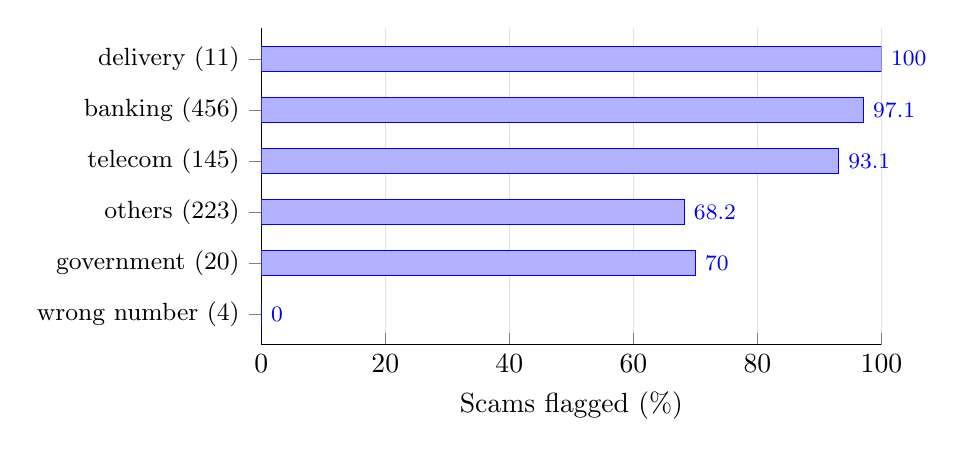
\begin{tikzpicture}
\begin{axis}[
  xbar, width=0.78\textwidth, height=5.6cm, xmin=0, xmax=100,
  xlabel={Scams flagged (\%)}, symbolic y coords={wn,gov,oth,tel,bank,del},
  ytick=data, yticklabels={wrong number (4),government (20),others (223),telecom (145),banking (456),delivery (11)}, y tick label style={font=\small}, nodes near coords, nodes near coords style={font=\footnotesize},
  bar width=9pt, enlarge y limits=0.12, xmajorgrids, grid style={black!12}, axis lines*=left,
  every axis plot/.append style={fill=deFill, draw=deLine}]
\addplot coordinates {(0,wn) (70.0,gov) (68.2,oth) (93.1,tel) (97.1,bank) (100,del)};
\end{axis}
\end{tikzpicture}
\caption{Fishing for Smishing, India: scams flagged by the reporters' scam type (campaigns in brackets). With the link
left out (the reports hide links), 86.3\% are still flagged.}
\label{fig:bytype}
\end{figure}

\textbf{What the numbers say.}
\begin{itemize}
  \item \textbf{Scams:} on real Indian scams Sajag had never seen, it flags 88\%: almost all banking, SIM-card and delivery
        scams. Most misses carry no link, no money and no deadline: ``Hey there! I am using WhatsApp.'', ``Hi, I'm Rahul,
        Project Manager at \dots'', a loan ``request accepted, check your loan amount''. Some reports are not scams at all
        (a Google verification code).
  \item \textbf{Normal messages:} 1.2\% are flagged in the public held-out set. In the India set it is 59\%, because the
        sheet's senders are typed names: with a real registered sender ID, 1 of 10 normal messages was flagged. The phone
        reads the real sender ID, so the number that counts is the real traffic below.
  \item \textbf{Titles:} of the 96 caught India scams, the alert's title names the right kind of scam for 52 (54\%), a
        general kind for 29 (30\%) and the wrong kind for 15 (16\%), mostly ``Fake bank KYC'' for reward-point and
        SIM-card scams: Sajag has no title of its own for SIM-card, loan or investment scams yet (Phase 2).
  \item \textbf{What the message says:} 89.6\% of caught India scams and 88.2\% of caught reported scams get at least one
        fixed phrase for Llama (prompt v5).
\end{itemize}

\subsection{The team's real messages}
\label{sec:real}

The hub's log holds what the app decided for every message the team's four phones forwarded; nothing is re-scored.
On 22 November every flagged message was labelled (scam, marketing or normal) except 14: 3,126 messages, 524 labelled.
Texts of SMS from phone numbers and of chats are kept only when flagged, so their missed scams cannot be counted;
every SMS from a registered sender ID is kept.

\begin{table}[H]
\centering\small
\begin{tabularx}{\textwidth}{@{}>{\raggedright\arraybackslash}X r r >{\raggedright\arraybackslash}p{3.6cm} r@{}}
\toprule
\textbf{Sender} & \textbf{Received} & \textbf{Flagged} & \textbf{Flagged: scam / marketing / normal} & \textbf{Normal per 100}\\
\midrule
SMS from a registered sender ID & 327 & 44 & 4 / 25 / 14 (1 not labelled) & \textbf{4.3}\\
SMS from a phone number & 17 & 12 & 3 / 1 / 8 & 47.1\\
Chat from an unknown number & 58 & 8 & 1 / 2 / 5 & 8.6\\
Chat from a saved contact (testing switch) & 2,723 & 243 & 50 / 61 / 119 (13 not labelled) & 4.4\\
All (with 1 SMS from a short code) & 3,126 & 307 & 58 / 89 / 146 (14 not labelled) & \textbf{4.7}\\
\bottomrule
\end{tabularx}
\caption{The team's real messages, as the app decided. Normal per 100: normal messages flagged per 100 received.}
\label{tab:real}
\end{table}

\begin{itemize}
  \item \textbf{False alarms on real messages: 4.3 normal SMS per 100 from registered sender IDs} (at most 4.6 if the
        one unlabelled flagged SMS is normal), and 4.7 per 100 over all 3,126 messages (at most 5.1).
  \item \textbf{The sender ID on real SMS}: of the labelled SMS, normal messages flagged fall from 94\% (text alone) to
        15\% (with the sender), marketing from 87\% to 19\%, while 7 of 8 scams (88\%) stay flagged.
  \item \textbf{Scams from registered sender IDs}: 4 flagged, 1 missed (a fantasy-league offer): the open door of
        Section~\ref{sec:limits}.
  \item \textbf{Most false alarms are group chats} seen through the testing switch (college notices with links, shared
        PDFs, links to sign-in pages), and personal SMS from phone numbers that carry a link or a number, which are weighed
        as risky on purpose.
\end{itemize}

\subsection{Live test on the phone}
\label{sec:live}

On 22 November a second phone sent 20 test messages (11 scams of different kinds, 9 normal) to the Galaxy S25 running
Sajag 3.2, as WhatsApp messages from a saved contact, first with the S25 on the hub's Wi-Fi, then 4 of the scams again
with its Wi-Fi off. The messages were written by us, so this tests that the whole app works, not its accuracy.

\begin{table}[H]
\centering\small
\begin{tabularx}{\textwidth}{@{}>{\raggedright\arraybackslash}p{3.0cm}>{\raggedright\arraybackslash}p{2.6cm}X@{}}
\toprule
\textbf{Round} & \textbf{Messages} & \textbf{Result}\\
\midrule
1, hub's Wi-Fi & 11 scams & \textbf{11 flagged} (9 dangerous, 2 suspicious); the title names the right kind for 9; the SIM-card and the reward-point scams were titled ``Fake bank KYC message'' (the gap found in Section~\ref{sec:acc})\\
1, hub's Wi-Fi & 9 normal & \textbf{8 safe}, no alert; 1 suspicious: ``Mom, I paid the electricity bill today, Rs 1,240'', the hard case on the list\\
2, Wi-Fi off & 4 scams again & \textbf{4 of 4 alerted again}, same verdicts: the phone alone, and a message sent twice gets two alerts\\
\bottomrule
\end{tabularx}
\caption{Live test on the Galaxy S25.}
\label{tab:live}
\end{table}

Every notification named the sender, the start of the message and the time it arrived. Two real bank debit SMS that
reached the S25 during the test were flagged suspicious: real false alarms of the kind Table~\ref{tab:real} counts.
Llama's explanations with prompt v5 are generated for the 87 graded cases and will be graded in Phase 2.

\subsection{Earlier message results}

\begin{table}[H]
\centering\small
\begin{tabularx}{\textwidth}{@{}>{\raggedright\arraybackslash}X>{\raggedright\arraybackslash}p{7.2cm}@{}}
\toprule
\textbf{Test} & \textbf{Result}\\
\midrule
Held-out public messages (1,816), the text model alone & F1 0.950; precision 0.941, recall 0.959; false alarms 1.27\%\\
India test set, text only & 94 of 100 scams flagged, but 48 of 75 normal messages too (64\%)\\
\emph{Projection}: every genuine India-set message with its ideal registered sender ID & 3 of 75 normal messages flagged (4\%)\\
First real SMS through the app (25 Oct) & an Airtel pack notice: 0.856 (dangerous) on its text alone, 0.106 (safe) with its real header \code{AE-AIRTEL-S}\\
The team's real traffic (2,674 messages, three phones, 14 Nov) & SMS from registered headers: 35 of 273 flagged (13\%), mostly marketing\\
Sender rules (226 messages from registered headers) & \emph{cap} and \emph{brand}: no false alarm added, switched on; \emph{suffix}: 7 more, left off\\
SMS model v2 against v1 (rule fixed in advance) & did not pass: fewer false alarms, but one registered-header scam missed\\
\bottomrule
\end{tabularx}
\caption{Message results before the accuracy test.}
\end{table}

\subsection{Links}

\begin{table}[H]
\centering\small
\begin{tabularx}{\textwidth}{@{}>{\raggedright\arraybackslash}X>{\raggedright\arraybackslash}p{6.4cm}@{}}
\toprule
\textbf{Test (held out by domain)} & \textbf{Result}\\
\midrule
Domain model alone & AUC 0.920\\
Brand-new phishing sites (not on any list), whole checker without the list & 80.9\% flagged, 69.7\% dangerous\\
Popular websites (Chrome UX Report top 1M) & 7.6\% flagged, 1.1\% dangerous\\
Held-out phishing sites with an Indian brand's name & 20 of 21 flagged\\
Popular \code{.in} websites & 0.3\% dangerous\\
\bottomrule
\end{tabularx}
\caption{Link checker. Real Indian scam short domains (\code{po9.in}, \code{kx3.in}) score safe on their own: they look like
genuine bulk-SMS link domains, so the sender, the text and the watch list decide.}
\end{table}

\subsection{Network}

\begin{table}[H]
\centering\small
\begin{tabularx}{\textwidth}{@{}>{\raggedright\arraybackslash}X>{\raggedright\arraybackslash}p{7.0cm}@{}}
\toprule
\textbf{Test} & \textbf{Result}\\
\midrule
CIC-IDS2017 (Monday learning, Tuesday--Friday attacks) & all 10 network-level attacks detected with the expected kind, 7 within the first minute; missed Heartbleed and 3 web attacks (no content is read); 144 false alarms in 40.7\,h, most of them beacons on the dataset's minute-rounded timestamps\\
Lab Wi-Fi, busy use, after the fixes & 0 false alarms in 20,960 flows (1.6\,h); before the fixes 5 in 4,415 flows\\
ESP32 test modes, live & DGA after about 30\,s, phishing look-up at once (and blocked), DNS tunnel after about 2\,min, beacon after about 10\,min\\
IoT-23 (real IoT malware, replayed) & 0 false alarms in 28.8\,h of three real smart-home devices; 2 of 5 infected devices flagged (4 of 10 labelled behaviours, both Mirai); missed Hakai, Torii and a trojan\\
DNS blocking on the Pi & self-test passed: answered, refused while blocked, answered again after unblocking\\
\bottomrule
\end{tabularx}
\caption{Network monitor.}
\end{table}

\subsection{Files}

21 of 21 harmless test files judged right (6 safe, 15 dangerous); no false alarm on 521 ordinary PDFs; of the team's 54
everyday files, 53 safe and 1 suspicious (a link in an e-book); 20\,ms per file on the Pi.

\subsection{Llama: speed and truthfulness}

\begin{table}[H]
\centering\small
\begin{tabularx}{\textwidth}{@{}>{\raggedright\arraybackslash}X>{\raggedright\arraybackslash}p{4.4cm}>{\raggedright\arraybackslash}p{4.4cm}@{}}
\toprule
 & \textbf{Raspberry Pi 4 (Cortex-A72)} & \textbf{Galaxy S25}\\
\midrule
Load the model & 13.7\,s (once, then resident) & 1.3\,s\\
Read the prompt & fixed prefix once (512 tokens, 38.5\,s), then only the case & 678 tokens in 2.0--2.6\,s\\
Write the answer & 3.3 tokens/s & about 36 tokens/s\\
A new explanation & 18--31\,s & 3.6\,s (5.2\,s with loading)\\
A repeated alert & at once (saved answers) & --\\
\bottomrule
\end{tabularx}
\caption{Llama 3.2 1B through ExecuTorch on the two Arm CPUs.}
\end{table}

\textbf{Are Llama's sentences true?} With prompt v4, Llama answered 100 different cases (89 flagged messages from the India
set, 11 network alert kinds), 183 sentences, graded blind by a team member as supported by the case, not supported, or
wrong. Of the 163 sentences users see after the grounding checks, \textbf{72\% were supported, 17\% not supported and 12\%
wrong}; all 16 network sentences were supported; the checks dropped 20 sentences, 19 of them unsupported or wrong. An AI
pre-check agreed with the human grader on 78\% of sentences (Cohen's $\kappa = 0.52$). Prompt v5's answers to the
same 87 cases are generated and will be graded in Phase 2; the numbers above are prompt v4's.

\subsection{Phone and hub agree}

\begin{table}[H]
\centering\small
\begin{tabular}{@{}lrrrr@{}}
\toprule
\textbf{Set} & \textbf{Messages} & \textbf{Identical} & \textbf{Same verdict} & \textbf{Same prompt}\\
\midrule
India test set, 9 senders each & 2,043 & 2,043 & 2,043 & 1,053 of 1,053\\
Public messages & 6,053 & 6,053 & 6,053 & 570 of 570\\
Edge cases, 8 senders each & 176 & 168 & 176 & 137 of 137\\
Links & 8,000 & 8,000 & 8,000 & 7,073 of 7,073\\
\bottomrule
\end{tabular}
\caption{Phone Guard (Kotlin) against the hub (Python), after prompt v5.}
\end{table}

\subsection{Resources on the Pi 4}

Over a 23-minute run with one explanation: the idle Pi used about 1\% CPU; the network monitor 0.1\% on average; the app
server 193--198\,MB; Llama 1,248\,MB resident, 4.1\% CPU on average and 96\% at peak while loading; available memory never
fell below 1,848\,MB of 3.7\,GiB; 39--74\,$^\circ$C; no under-voltage.

% ================================================================= 8
\section{An external review, and what we did with it}
\label{sec:review}

On 14 November an external reviewer read the whole project and wrote a hard 32-page review with a research plan. We agreed
with most of it, checked its claims against the code, and turned it into seven updates (36--42) before this report:

\begin{table}[H]
\centering\small
\begin{tabularx}{\textwidth}{@{}>{\raggedright\arraybackslash}p{5.2cm}X@{}}
\toprule
\textbf{The review said} & \textbf{What we did (update)}\\
\midrule
Any device on the Wi-Fi could use the hub's API & a pairing token on every request, limits on wrong tokens, a separate device token for the ESP32 (36)\\
Some numbers were projections, not measurements & every projection marked as such; the SMS model refuses to start as the sample model; the README rewritten around measured numbers (36, 40)\\
A scam from a registered sender ID is the open door & sender rules (\emph{cap}, \emph{brand}, \emph{suffix}) measured on real headers, two switched on (37, 38)\\
Llama's sentences were never checked for truth & grounding checks, and 100 answers graded sentence by sentence, with a second look and agreement statistics (38--38d)\\
Plain HTTP between phone and hub & HTTPS with a certificate the phone pins when pairing (39)\\
The hub kept message texts from every phone & a study switch per phone; texts only with it on, digits masked (39)\\
Detection without protection & DNS blocking for the whole home, with an automatic undo (40)\\
IoT malware claims untested on real malware & IoT-23 replay of real IoT malware captures (40--42)\\
\bottomrule
\end{tabularx}
\caption{The external review and our response in Phase 1.}
\end{table}

What the review asked for that Phase 1 could not finish is in the Phase 2 plan: a second human grader and non-expert users
for Llama's explanations, TRAI's header registry, a learned network classifier beside the rules with lists of known
controllers, a whole day of false-alarm measurement, protection for devices that bypass the hub's DNS, and more of the
team's labelled messages.

% ================================================================= 9
\section{Phase 1: what is done}
\label{sec:phase1}

\begin{table}[H]
\centering\small
\begin{tabularx}{\textwidth}{@{}>{\raggedright\arraybackslash}p{4.6cm}X>{\raggedright\arraybackslash}p{1.5cm}@{}}
\toprule
\textbf{Part} & \textbf{State} & \textbf{Updates}\\
\midrule
Message checker (SMS, chats, sender IDs) & running on the hub and on the S25; measured (Section~\ref{sec:acc}) & 1--9, 33--37, 43, 47\\
Link checker and phishing list & running; measured on held-out domains & 9, 27\\
File checker & running; measured on test files, 521 PDFs and everyday files & 29--32\\
Network monitor (rules, DNS, DGA, normal, beacons) & running on the hub; CIC-IDS2017, lab Wi-Fi and IoT-23 & 10--28, 40--42\\
Messages meet traffic; DNS blocking & running on the hub; self-test passed & 21, 40\\
Llama 3.2 1B on the Pi 4 (own C++ engine) & running; speed measured; 100 answers graded & 1--4, 17--19, 38\\
Phone Guard (checks on the phone) & running on the S25; identical to the hub on 16,272 messages & 43\\
Llama on the phone (ExecuTorch Android) & running on the S25; 3.6\,s per explanation & 44, 45\\
App Sajag 3.2 (screens, alerts, set-up) & running on the S25 & 46--48\\
Prompt v5 (what the message says) & running; parity checked; its answers to be graded in Phase 2 & 47\\
Security and privacy (token, HTTPS pinning, study switch) & running & 36, 39\\
Learning loop (log, labels, model v2, export, parity) & built and run once; v2 did not pass, v1 kept & 5, 24--25, 33--35, 43\\
ESP32 lab IoT device & four harmless test modes, all caught live & 14--16\\
Accuracy test & labelled sets, the team's real messages and the live test done; Llama v5 grading in Phase 2 & 49, 52\\
Repository organised by part (home hub, phone app, IoT device) & public on GitHub & 50, 53\\
\bottomrule
\end{tabularx}
\caption{The state of every part at the Phase 1 submission.}
\end{table}

% ================================================================= 10
\section{Limitations}
\label{sec:limits}

\begin{itemize}
  \item \textbf{Away from home the phone is on its own}: its verdicts, steps and explanations are the hub's, but without
        the 392,000-site phishing list and the file checker, which stay on the hub until the phone is back.
  \item \textbf{The text model learned from public data.} With text alone it flags many normal Indian messages; the real
        sender ID fixes much of that (normal SMS flagged fall from 94\% to 15\% on the team's labelled messages), but 4.3
        normal SMS per 100 from registered headers are still flagged, and more marketing ones.
  \item \textbf{A scam from a registered header is the open door.} The sender rules close part of it; v1 let through 3 of
        the 4 such scams on the team's phones.
  \item \textbf{Titles}: 16\% of caught scams get the wrong kind in the title (Section~\ref{sec:acc}).
  \item \textbf{Llama is slow on the Pi 4} (18--31\,s), and about one sentence in eight that users saw was judged wrong
        with prompt v4 by our one grader. The verdict and the steps never wait for Llama.
  \item \textbf{The network monitor reads no content}: web attacks and exploits pass unseen, and so does quiet malware on
        web ports (3 of 5 infected IoT-23 devices raised no alert). Encrypted DNS hides the names the DNS checks need.
        A device that joins already infected is learned as normal.
  \item \textbf{The monitor and the DNS block see only devices on the hub's hotspot}; a real home would put the hub in
        front of its router or make it the home's DNS server.
  \item \textbf{Installing the app}: Play Protect blocks side-loaded apps with SMS permissions, so it is installed from
        Android Studio; a public release needs Google's SMS permission approval.
  \item \textbf{Not measured yet}: a whole day of false alarms on the lab Wi-Fi, and a second person grading Llama.
\end{itemize}

% ================================================================= 11
\section{Phase 2 plan (until 5 February 2027)}
\label{sec:phase2}

Phase 2 grows the loop of Section~\ref{sec:approach}: more people's messages make a better model and better explanations,
in more languages, on every phone.

\subsection{More data, and models trained on it}
\begin{itemize}
  \item \textbf{More labelled Indian messages}: every phone in the study, labelled blind in the hub's terminal; the
        independent Fishing for Smishing reports and new public Indian sets kept as untouched test sets.
  \item \textbf{SMS model v3}: the three-class model retrained on the larger set, judged by the same rule fixed in
        advance; then a small multilingual encoder (an Indic BERT-style model, distilled and quantised to INT8) exported
        with ExecuTorch for the phone, compared with v3 the same way.
  \item \textbf{A scam-type model} trained on labelled types, to fix the wrong titles, with new types and playbooks for
        SIM-card, loan, investment and trading-app scams, fake customer care, UPI collect requests and SIM swap.
  \item \textbf{Personal models with privacy}: each household's hub fine-tunes on its own members' messages; next,
        federated training, where phones and hubs share model updates instead of texts, with differential privacy.
  \item \textbf{Sender IDs checked against TRAI's header registry}, with each header's owner: the strongest answer to
        scams from registered headers.
\end{itemize}

\subsection{Better explanations}
\begin{itemize}
  \item \textbf{Prompt v5 graded against v4} on the same 87 cases, whose answers are already generated on the Pi, by two
        graders.
  \item \textbf{Llama 3.2 3B on the phone} (about 3.7\,GB while running: it fits the S25, not the Pi 4), still through
        ExecuTorch on the Arm CPU, chosen by a rule fixed in advance: fewer wrong sentences on the same graded cases, at an
        acceptable time per explanation.
  \item \textbf{Fine-tuning Llama} (LoRA) on graded explanations, so that the style and the facts need fewer examples
        in the prompt.
  \item \textbf{Grading by a second person and by non-expert users}: do the sentences help people act?
  \item \textbf{A daily safety digest} written by Llama from the day's alert kinds and counts.
\end{itemize}

\subsection{More languages}
\begin{itemize}
  \item Explanations and steps in Hindi everywhere (Llama already explains Hindi messages in Hindi), then Bengali,
        Tamil, Telugu, Marathi and Gujarati, and code-mixed Hinglish messages; the rules' patterns in those scripts.
  \item The explanation read aloud (text-to-speech on the phone) for users who do not read easily.
\end{itemize}

\subsection{Wider protection}
\begin{itemize}
  \item \textbf{The phone as complete as the hub}: the phishing list copied to the phone when home, files checked on the
        phone, and the phone's own connections checked and blocked through a local VPN.
  \item \textbf{Network}: a learned flow classifier beside the rules, trained on more than one dataset; a rule for many
        unanswered tries at one internet address and lists of known controllers (the IoT-23 misses); a whole-day
        false-alarm measurement; one-tap quarantine of a device; DNS for devices that bypass the hub.
  \item \textbf{Scam calls}: the PS3 area we do not cover yet, starting from caller IDs and the call log.
  \item \textbf{Hardware}: a Raspberry Pi 5 (CPU only, or with the AI HAT+ through HailoRT as a separate, documented
        pipeline as PS3 allows, with Llama staying on the Arm CPU); battery and heat measured on the phone.
\end{itemize}

\begin{table}[H]
\centering\small
\begin{tabularx}{\textwidth}{@{}>{\raggedright\arraybackslash}p{3.0cm}X@{}}
\toprule
\textbf{When} & \textbf{Milestone}\\
\midrule
December 2026 & all study phones labelling; SMS model v3 and the scam-type model; second grader; Hindi steps\\
Early January 2027 & Llama 3.2 3B on the phone, compared; phishing list and files on the phone; TRAI header list\\
Late January 2027 & multilingual encoder on the phone; federated training prototype; network classifier; whole-day measurement\\
5 February 2027 & Phase 2 PoC: report, video and the measured comparisons\\
\bottomrule
\end{tabularx}
\caption{Phase 2 timeline.}
\end{table}

% ================================================================= 12
\section{The repository: where each part lives}
\label{sec:repo}

The code is public at \repourl. Its folders follow the parts of Sajag described in this report: the Home Hub
(Section~\ref{sec:arch}), the phone app (Section~\ref{sec:phone}) and the IoT lab device, then the results, the guides
and this report. A reviewer can start from the README's ``Start here'' table, and every part's folder has its own README.

\begin{keybox}[title=How the repository is organised]
\small
\begin{verbatim}
ps3-guardian-arm/
├── home-hub/           The Home Hub: everything that runs on the Raspberry Pi 4
│   ├── app/            the hub's server and web page, HTTPS, DNS blocking
│   ├── detectors/      the checkers: sms/, url/, files/, net/
│   ├── advisor/        playbooks, prompts, Llama service, grounding checker
│   ├── llama-engine/   Llama's export with ExecuTorch, our C++ engine
│   ├── scripts/        set-up, services, downloads, measuring tools
│   └── tests/          379 automated tests
├── phone-app/          Sajag for Android: Phone Guard and Llama on the phone
├── iot-lab-device/     the ESP32 lab IoT device and its simulation
├── results/            every measured result, and how to reproduce it
├── docs/               guides: install, use and test each part
└── report/             this report (PDF and LaTeX)
\end{verbatim}
\end{keybox}

\begin{table}[H]
\centering\small
\begin{tabularx}{\textwidth}{@{}>{\raggedright\arraybackslash}p{4.3cm}>{\raggedright\arraybackslash}p{3.4cm}X@{}}
\toprule
\textbf{Folder} & \textbf{What it is for} & \textbf{With it you can}\\
\midrule
\code{home-hub/app/} & the hub's entry point: the server the phone and the page talk to & check a message, link or file from the page or the app; see alerts and devices; block and unblock websites; give a paired phone the Llama files\\
\code{home-hub/detectors/} & the checkers (Section~\ref{sec:algo}) & judge messages and sender IDs (\code{sms/}), links (\code{url/}), files (\code{files/}) and every device's traffic (\code{net/}); train and evaluate their models\\
\code{home-hub/advisor/} & advice and explanations (Section~\ref{sec:llama}) & turn a finding into the playbook's steps at once and Llama's checked explanation after; grade Llama's sentences\\
\code{home-hub/llama-engine/} & Llama on the Pi 4 (Section~\ref{sec:engine}) & export Llama 3.2 1B with ExecuTorch and build the C++ engine for the Cortex-A72\\
\code{home-hub/scripts/} & running and measuring the hub & make the Pi a hotspot, install the services, set up DNS blocking, download the lists, measure real traffic, export the checks to the phone, run the accuracy test\\
\code{home-hub/tests/} & keeping it correct & run 379 tests on a laptop: \code{python -m pytest}\\
\code{phone-app/} & protecting each person anywhere (Section~\ref{sec:phone}) & build Sajag in Android Studio and install it on a phone; Phone Guard is in \code{guard/} and its data in \code{assets/guard/}\\
\code{iot-lab-device/} & showing the hub catch an infected IoT device & flash the ESP32 and start its four harmless test modes from the hub's page\\
\code{results/} & how well it works (Section~\ref{sec:results}) & read every measured number with the command that reproduces it\\
\code{docs/} & how to use each part & follow the guides: the app and pairing, Phone Guard, the network monitor, DNS blocking, the ESP32, the tests\\
\code{report/} & the written submission & read or rebuild this report (\code{xelatex})\\
\bottomrule
\end{tabularx}
\caption{What each folder is for.}
\end{table}

\textbf{To run it.}
\begin{itemize}[leftmargin=*]\raggedright
  \item On a Raspberry Pi, from \code{home-hub/}: the hotspot (\code{scripts/setup\_gateway.sh}); the app server and
        Llama (\code{scripts/install\_service.sh}); the network monitor (\code{scripts/install\_netmon.sh}); DNS blocking
        (\code{scripts/setup\_dns\_block.sh}).
  \item On a laptop, from \code{home-hub/}: \code{pip install -r requirements.txt}, then \code{python -m pytest}.
  \item The app: open \code{phone-app/} in Android Studio, run it on the phone, and pair it with the hub in the set-up.
  \item Branches: \code{main} holds the Phase 1 submission, \code{dev} the work for Phase 2; the tag
        \code{phase1-submission} marks the submitted version.
\end{itemize}

% ================================================================= 13
\section{Conclusion}

Sajag shows that a home hub and a phone, both on Arm, can protect a household from scams, phishing and IoT threats with
no cloud: small checkers decide in milliseconds, playbooks give the steps at once, and Llama 3.2 1B through ExecuTorch
explains each alert in plain words, held to its evidence, in 3.6\,s on a phone or 18--31\,s on a Raspberry Pi 4. On real
Indian scam reports it had never seen, it flags 88\%. The hub protects every device at home; each phone protects its owner
anywhere; and each person's messages, fed back to the hub with consent, are how the next model will learn what one public
dataset cannot teach it. Phase 2 will grow that loop: more data, better models, better explanations, and more of India's
languages.

% ================================================================= references
\section*{References}
\addcontentsline{toc}{section}{References}
\small
\begin{enumerate}[label={[\arabic*]}, leftmargin=*, itemsep=1pt]
  \item Arm Education. \emph{Arm Bharat AI-SoC Student Challenge 2026--27}, problem statements and rules.
        \url{https://arm-education.github.io/Arm-Developer-Labs/Bharat_AI_SoC_2026_27.html}
  \item Meta. \emph{Llama 3.2} model card and licence (1B Instruct, SpinQuant INT4), 2024.
  \item Z. Liu et al. \emph{SpinQuant: LLM quantization with learned rotations}. arXiv:2405.16406, 2024.
  \item PyTorch. \emph{ExecuTorch}: on-device inference for PyTorch models, release 1.5, with the XNNPACK backend.
  \item Z. Aouini and A. Pekar. \emph{NFStream: a flexible network data analysis framework}. Computer Networks, 2022.
  \item I. Sharafaldin, A. H. Lashkari and A. A. Ghorbani. \emph{Toward generating a new intrusion detection dataset and
        intrusion traffic characterization} (CIC-IDS2017). ICISSP, 2018.
  \item S. Garcia, A. Parmisano and M. J. Erquiaga. \emph{IoT-23: a labeled dataset with malicious and benign IoT network
        traffic}. Stratosphere Laboratory, 2020.
  \item T. A. Almeida, J. M. G. Hidalgo and A. Yamakami. \emph{Contributions to the study of SMS spam filtering}
        (SMS Spam Collection). DocEng, 2011.
  \item S. Mishra and D. Soni. \emph{SMS phishing dataset for machine learning and pattern recognition}. Mendeley Data, 2022.
  \item A. Prasad and S. Chandra. \emph{PhiUSIIL: a diverse security profile empowered phishing URL detection framework}.
        Computers \& Security, 2024.
  \item Phishing.Database: active phishing domains, \url{https://github.com/mitchellkrogza/Phishing.Database}.
  \item Chrome UX Report top sites lists, \url{https://github.com/zakird/crux-top-lists}.
  \item A. Agarwal, A. Papasavva, G. Suarez-Tangil and M. Vasek. \emph{Fishing for Smishing}. ACM IMC, 2025. Dataset (CC BY 4.0):
        \url{https://github.com/reportsmishing/Smishing-Dataset-IMC25}
  \item ExtraHop. DGA training data (MIT licence).
  \item Telecom Regulatory Authority of India. \emph{Telecom Commercial Communications Customer Preference Regulations},
        2018, and the URL whitelisting direction of 2024.
  \item Reserve Bank of India. Banks' websites under the \code{.bank.in} domain, 2025.
  \item F. Pedregosa et al. \emph{Scikit-learn: machine learning in Python}. JMLR, 2011.
  \item E. B. Wilson. \emph{Probable inference, the law of succession, and statistical inference}. JASA, 1927.
  \item J. Cohen. \emph{A coefficient of agreement for nominal scales}. Educational and Psychological Measurement, 1960.
  \item National Cyber Crime Reporting Portal (\url{https://cybercrime.gov.in}) and helpline 1930.
\end{enumerate}
\normalsize

% ================================================================= appendix
\appendix
\section{Timeline}

\begin{table}[H]
\centering\small
\begin{tabularx}{\textwidth}{@{}>{\raggedright\arraybackslash}p{2.6cm}X@{}}
\toprule
\textbf{2026} & \textbf{Milestone}\\
\midrule
25 September & plan: fast checkers feeding a Llama advisor, sized for the Pi 4\\
19--23 October & SMS baseline; message $\to$ finding $\to$ advice $\to$ app; Llama exported with ExecuTorch and run on the Pi 4; the fast advisor\\
24--26 October & India test set; sender-aware scoring; the Android companion; chats; link checker; network detector on CIC-IDS2017\\
31 Oct -- 5 Nov & the Pi becomes the hotspot; the ESP32 lab device; Llama explains network alerts; devices and scam-link fusion; measurement tools; lab false alarms fixed\\
7--13 November & the file checker (asked for by our mentor)\\
14--16 November & SMS model v2 tested (kept v1); the external review; security, sender rules, Llama grading, HTTPS, study switch, DNS blocking, IoT-23\\
21--22 November & Phone Guard and Llama on the phone; the app becomes Sajag; prompt v5; the accuracy test\\
\bottomrule
\end{tabularx}
\caption{Phase 1 in 53 updates.}
\end{table}

\end{document}
